\documentclass{article}
%\usepackage{minted}
\usepackage[backend=bibtex,style=numeric, citestyle=ieee]{biblatex}
\addbibresource{bibliography.bib}
\usepackage{pdfpages}
\usepackage{amsmath}
\usepackage[ruled,vlined]{algorithm2e}
\usepackage{pgfgantt}
\usepackage[noend]{algpseudocode}
\usepackage{graphicx}
\usepackage{float}
\usepackage{hyperref}
\usepackage{titlesec}
\usepackage{longtable}
\usepackage[
top    = 2.50cm,
bottom = 2.50cm,
left   = 2.75cm,
right  = 2.75cm]{geometry}

\newcommand{\CS}{C\nolinebreak\hspace{-.05em}\raisebox{.6ex}{\tiny\bf \#}}
\begin{document}



\pagenumbering{roman}
\begin{titlepage}
	\begin{center}
		
		  	
\includegraphics[width=0.5\columnwidth]{images/nottingham-logo.png}
		
		\vskip 1in 
		\par 
		\LARGE {\bf A Data-Driven Approach To Bus Timetable Optimisation Recommendations.}
		
		\vskip 0.5in \par
		\large {Submitted June 2021, in partial fulfillment of \\ the conditions for the award of the degree MSci Computer Science.}
		

		\vskip 0.3in \par
		\large {\bf Jonathan Foot} \\
		
		\large { School of Computer Science \par
		University of Nottingham}
		
		
		\vskip 0.3in \par
		\large {\bf Supervised by Dr Jason Atkin}
		\vskip 0.3in \par
	
		
		\vskip 0.5in \par
		\normalsize {I hereby declare that this dissertation is all my own work, except as indicated in the text. }
		
		\vskip 0.5in 
		\normalsize {Signature : Jonathan Foot}
		
		\vskip 0.1in
		\normalsize {Date 04/05/2021}
		
		
		\vskip 0.4in \par
		\normalsize {I hereby declare that I have all necessary rights and consents to publicly distribute this dissertation via the University of Nottingham's e-dissertation archive.}
		
			
	
	\end{center}
\end{titlepage}

\newpage

\addcontentsline{toc}{section}{Abstract}

\setlength{\parskip}{1em}



\section*{\centering{Abstract}}

In this dissertation, I explored using several months worth of historical bus journey data to feed a search algorithm on three main optimisation criteria, with the goal that the program could be used by a bus operator to aid with improving their timetables during a review period. More data than ever before is being recorded about buses within the UK and this provided an exciting opportunity to encourage greater usage of buses, for the benefits they provide. 

\par
The first optimisation criteria was minimising unneeded slack time and travel times while balancing the percentage of buses predicted to be on time. The second optimisation criteria was to maximise cohesion between services that share a common route segment, by ensuring they are more spread out at shared stops. A shared route segment is defined as ``N'' consecutive stops shared by two or more services, where ``N'' is the minimum segment length. The third optimisation target is to minimise change as much as possible, as too many changes at once make it very difficult to predict how it is likely to perform in the real world. The search algorithm used is tabu-search coupled with squeaky wheel optimisation for a more targeted and informed search. I have demonstrated that tabu-search and squeaky wheel optimisation can be used to optimise a buses timetable to great effect. 


	
\vspace{5em}

\addcontentsline{toc}{section}{Acknowledgements}

\section*{\centering{Acknowledgements}}

I would like to thank my academic supervisor, Dr Jason Atkin, for all his guidance and support throughout the academic year.

\setlength{\parskip}{0em}


\newpage

\tableofcontents


\newpage

\setcounter{page}{1}
\pagenumbering{arabic}
% Do all this to reduce the page count ;) 

\titlespacing\section{0pt}{12pt plus 4pt minus 2pt}{0pt plus 2pt minus 2pt}
\titlespacing\subsection{0pt}{12pt plus 4pt minus 2pt}{0pt plus 2pt minus 2pt}
\titlespacing\subsubsection{0pt}{12pt plus 4pt minus 2pt}{0pt plus 2pt minus 2pt}
\setlength{\parindent}{2em}
\setlength{\parskip}{1em}
\setlength{\belowcaptionskip}{-10pt}


\section{Introduction and Motivation}


Bus transit systems remain the UK's leading public transportation method, with the average UK resident making 48 trips annually \cite{RN9}. Bus networks allow for a relatively low initial infrastructural investment while offering great adaptability and environmental benefits; particularly with the popularity of hydrogen, electric and bio-gas buses increasing. Although, private transportation methods still remain the UK's preferred method of transport, with the average person taking 602 trips by car \cite{RN9}, over 12 times that of the number of bus trips. 

\par
One of the leading deterrents for greater adoption of bus transportation is ``a belief that buses cannot be relied on to stick to their timetables''\cite{RN10}. Transport operators are responsible for the network route design, setting the frequencies, timetables and assigning vehicles and drivers to trips. When creating the timetable operators must consider both external factors, such as traffic, roadworks, severe weather, sporting events and internal factors, such as delays from previous trips affecting the subsequent trips and delays on passenger boarding and alighting \cite{RN11}.

\par
The UK Senior Traffic Commissioner's guidelines are for 95\% of buses to be ``on-time'', which is defined as departing between 1 minute early to 5 minutes late at a timing point, or arriving 5 minutes or later at the final destination point.\cite{RN14}. If bus operators repeatedly fail to adhere to this guideline, they can be fined up to £550 per vehicle \cite{RN14}.  A timing point is a special type of bus stop that must normally appear at least every 15 minutes in a services schedule and is one where the bus is not allowed to leave until the scheduled time.

\par
 One way to ensure compliance is to add a significant amount of excess wait times at stops to recoup for any delays. But this will increase journey times and unneeded waiting can be considered ``dead time'' where the bus operator is not making any money. Creating a reliable timetable is therefore important to both the operators and customers alike.


\par
98\% of buses in Great Britain are equipped with automatic vehicle location (AVL) devices\cite{RN12}, which is used to monitor the punctuality of buses to a high degree of accuracy. With some operators even storing the exact longitudinal and latitudinal position of every bus, up to every 30 seconds. There is more data about buses than ever before and with the United Kingdom Government legislating the Bus Service Act 2017\cite{RN13}, bus open data is becoming increasingly more accessible. I have used this open-data to drive an optimisation algorithm to make new timetable recommendations, improve average on-time performance and instil greater customer confidence in bus timetables and using buses as a form of transport.



\section{Related Work}
There is already a plethora of work on public transit systems, which can be categorised into five key parts \cite{RN18} \cite{RN20}: transportation route network design (TRND); timetable setting; crew scheduling; vehicle scheduling; real-time control during service. Timetable setting has further been summarised into following optimisation objectives\cite{RN7}: minimising average wait time; minimising transfer times between routes; minimising total travel time; balancing of operators cost with users benefits. 

 \par
Transportation route network design involves defining each line's route, length, stop density and key defining characteristics, such as proposed general frequency. Timetable setting defines when each bus will leave the first bus stop and takes into consideration the uncertainty of passengers' demands and travel times, due to external and internal factors\cite{RN11}. Considerations should also be made for connections between other lines, train times, school times, \textsl{et al}. This can be even further complicated by having multiple bus depots, (often referred to as the Multiple Depot Vehicle Scheduling Problem), considerations for staff changeover locations and breaks, minimisations of dead-heading travels (any driving when the bus is not on a passenger-carrying journey), utilisation of bus-lanes and bus-gates, unplanned vehicle maintenance, roadworks and changes in fuel prices. 

\par 
Setting and evaluating a bus timetable can therefore be described as an NP-Hard problem \cite{RN15}, because of the complex nature of having so many inter-connected multi-objective requirements. Due to this, many people choose to target only one or two aspects of the problem at a time; as it is believed impractical that a single algorithm could consider all possible factors and generate a perfect new timetable.


\par
Data-driven approaches have only started being researched relatively recently, which I suspect is because the quality and accessibility of the data has only become viable in the last decade, with 2010 being the first year where over half of buses in the UK had AVL\cite{RN12}. As such, there is a limited number of papers on my exact proposal.

\par
 One such paper however is proposed by Jinjun Tang \textsl{et al} who used a multi-objective genetic algorithm \cite{RN18}, to minimise the passenger waiting time, whilst also reducing the total number of departures. This ensures that the number of vehicles needed to operate the service during peak times is not significantly greater than non-peak times, for greater utilisation of vehicle resources. Like me they proposed a data-driven approach, however, they used Smart Card and GPS Data to understand passenger demand and travel times. Furthermore, they added vehicle capacity as one of their constraints.

\par
Fangzhou Sun \textsl{et al} proposed a single-objective greedy and genetic algorithm (GA)\cite{RN8}, to increase a services' on-time percentage by minimising slack times. With the constraint that the last time point of a trip must always be the first time point of the next i.e., every trip must follow on from the last. Like me they are also using a data-driven approach using historical time-point and schedule data. However, unlike me they assume that the arrival and departure time will always be the same, so no consideration for boarding time is made and they proposed a GA something I chose not to do. They found that a GA was more effective than a Greedy algorithm.  

\par
Sanchita Basak \textsl{et al} similarly proposed a single-objective optimisation task, with a greedy, genetic and Particle Swarm Optimisation algorithm (PSO), with the ``objective of maximizing [the] probability of bus arrivals at time points with delays within desired on-time ranges''\cite{RN7}, using historical time-point data and real-time information. Unlike the other two data-driven approaches they focused more on the seasonal difference and monthly grouping of patterns throughout the year. They also discovered that a PSO executed faster than a GA, while producing similar results. Their optimisation targets were similar to my own, but their method very different, I also made no account for grouping seasonal trends.


\par 
Friedman proposed one of the earliest timetable scheduling solutions in 1975\cite{RN22} , representing the problem as a mathematical programming model, with the aim to minimise average passenger waiting time; considering constraints on allocations of drivers and vehicles. Although he relied upon known deterministic conditions such as passenger numbers and traffic intensity, an unrealistic assumption to make.

\par 
Daniel Sun \textsl{et al} used a heuristic algorithm to look at how different capacity buses could be used to deal with demand fluctuations  \cite{RN32}. Ceder and Lucas, looked at creating a timetable to minimise bus overcrowding \cite{RN33}. Yinghui Wu \textsl{et al} proposed an integer-programming model and a genetic algorithm with a local search to optimise the slack times in a timetable and reduce randomness \cite{RN26}, by focusing on three types of passengers, those transferring, boarding and currently travelling. Some have attempted optimising the TRND and timetables simultaneously with a GA to minimise travel and transfer times \cite{RN23}\cite{RN31}. 
 

 
\subsection{Under-researched areas}
 
While there is already a lot of research and proposed methods into the different areas of timetable optimisation. One area which has not been focused upon as much is considerations for routes that share the same common path for a portion of their routes before separating off. This is particularly common for urban areas, where local councils may have invested into bus lanes, bus gates or less popular sump busters. Due to the road space invested into them and their ability to reduce travel times \cite{RN34}, they lend themselves to encourage multiple services to share the same route-segment. These shared route-segments across several services have been coined ``bus corridors'' by some.

\par
When multiple services share a common route-segment, passengers may not be concerned about which of the services they board on, if they do not wish to travel past their shared segment. Instead, they will choose to travel on whichever service arrives first at their stop. It is this phenomenon I wish to explore further.


\section{Description of the work}

I intend to create a program that will produce an improved optimised timetable for bus-operators, to use internally during their timetable reviews and enable them to make more informed decisions. It shall do this by taking in a set of historical timetables and vehicle times data and then using this data to optimise the timetables based upon three optimisation criteria. 


\par
The program will let the bus-operator review their services' current performance metrics such as percentage on-time performance (also known as time point schedule adherence) and cohesion with other services which share a common route-segment. The program will let them select a service and choose to optimise it.

\par
Once selected the program will ask the bus-operator to input in a time period of interest, and it will then find all of the different timetables that operated within this period. For example, a service might have a different Sunday timetable to its weekday timetable, or its weekday timetable may have changed mid-way through the year. Once the different timetables have been identified the bus-operator can select one timetable to optimise. It is assumed that the performance of the timetable last year will remain generally consistent the following year and this will account for seasonal differences. 

\par 
The selected bus service's timetable acts as the ``primary service'' of the search, for which other linked services can be optimised with. The program will do this by making suggestions for other services that share a common route-segment with the primary service. The user can then select none or several of the suggested services, to include in the search and also optimise their timetables, enabling better cohesion between them. By making services at a stop more uniformly spread out and less crowded.


\par
Finally, it will give a higher ``score'' to a solution with the fewest number of changes, this is to prevent an overzealous solution and because it is difficult to be able to confidently predict how it is likely to perform. The user is then asked to order the optimisation targets based on importance and can change key parameterised values. The program will then execute and return a set of new optimised timetables, along with a predicted set of performance metrics to allow for comparison against the previous timetable.

\subsection{Optimisation Criteria}
The three optimisation targets can therefore be summarised as:
\begin{itemize}
	\item Minimise the unneeded slack (dwell) time at timing points and the travel times at every stop while balancing the percentage of buses predicted to be ``on-time''.  
	\item Minimise the number of total changes and the severity of the changes, aiming to keep the timetable as close to the original as possible. Too many changes at once make it very difficult to be able to reliably predict how it is likely to function. 
	\item Maximise the uniform distribution of different services arriving at the same stop, by spreading out headway times. This requires identifying routes that share a common route-segment.
\end{itemize}
 
 The importance/ weighting (pareto dominance) of the three optimisation targets will be parameterised, such that the user can optimise a timetable based on what is most important to them, or to experiment with several timetable ideas. This is because the program will produce a pareto solution, to have the highest percentage of on-time buses you would need to increase the slack time. Similarly, to have an even distribution of services at a stop you might need to add excess slack time.
 
 
\subsection{Aims and Objectives}
The aims and objectives of this project are:
\label{aimsObjectivs}
\begin{enumerate}
	\item Interface with the Reading Buses Open Data API, request and download data required from the API.
	\item Search through the data and identify points where the timetables changed.
	\item Generate the performance metrics, such as average on-time performance of the old timetable for the previous year.
	\begin{enumerate}
		\item Use these metrics, to compare and contrast against the new timetable later. 
	\end{enumerate}
	\item Take in the historic vehicle data and generate a new optimised timetable, to the minute accuracy.
	\begin{enumerate}
		\item Explore multiple different methods for timetable optimisation.
		\item The new timetable will try to minimise unneeded idle/dead slack time at timing points.
		\item The new timetable will try to ensure that the journey times are realistic between stops at the time of day.
		\item The new timetable will not consider constraints on the number of vehicles, or drivers availability. 
		\item The new timetable will not consider how these changes might affect connections between other routes.
		\item The new timetable must bear some resemblance to the original headway times and will be restricted to prevent an overzealous solution.  
		\item The new timetable cannot alter the bus services route design.
		\item The optimisation strategy must consider the times of other services, which share a common route-segment.
		\item The optimisation algorithm should allow for the parameters and constraints to be edited by the end-user.
	\end{enumerate}
	\item Produce a simulation/scoring system that can take in the proposed timetable to allow for comparison with the original timetable.
	\item Create a user-friendly GUI, which can graphically highlight the differences between the two timetables, to easily distinguish where the improvements have been made.  
\end{enumerate}


\section{Design and Methodology}

In the following section, I will outline the overall design of the program, both from the end-user's perspective, with the GUI and parts of the internal system, such as data-schemas, technologies chosen and algorithm designs.


\subsection{Chosen Technologies}
For this project, I have chosen to use \CS \ .NET 5, with Visual Studio 2019 Enterprise. This is because \CS, particularly with the latest .NET version offers the speed and versatility required to be able to quickly process large volumes of data. Whilst also being syntactically an easy language to develop in. Particularly with the use of LINQ, which allows me to be able to declaratively query complex data structures with ease. Visual Studio also offers industry-leading debugging tools to speed up development further. Moreover, it is my strongest programming language and as such, I can be confident in my proposed implementation strategies and estimated timelines.

\subsection{Graphical User Interface}

Figure ~\ref{fig:gui1} and ~\ref{fig:gui2} show my GUI designs, I have focused upon creating a functional, easy to use and intuitive program layout. The final produced GUI remained similar to this design, but with minor changes to improve usability.

\begin{figure}[H]
	\centering
	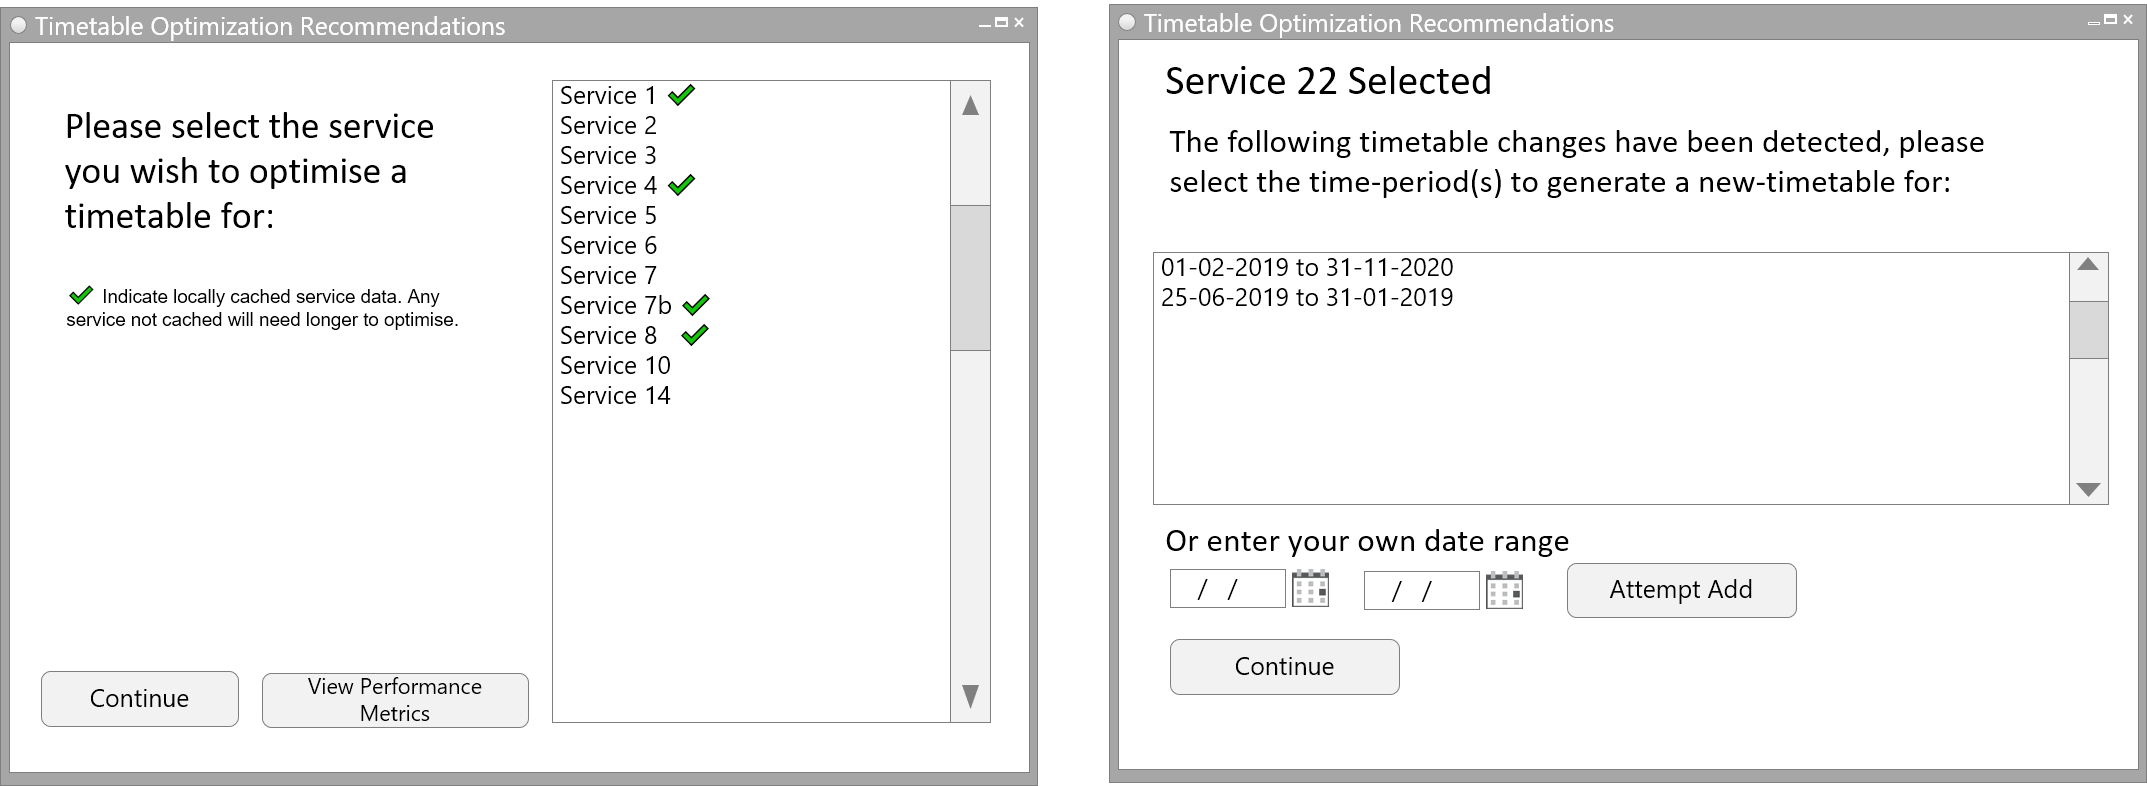
\includegraphics[height=105px]{images/GUI_1.png}
	\caption{GUI Design for Screens 1 to 3.}
	\label{fig:gui1}
\end{figure}

The start screen lets the user select the service they want to generate a new timetable for (or to view its current performance metrics), the second screen lets the user select a time-period for when the new timetable would be in effect for. The third screen lets the user see routes that share common-route segments with their selected route and can then optimise several timetables concurrently to harmonise their coordination. 


\begin{figure}[H]
	\centering
	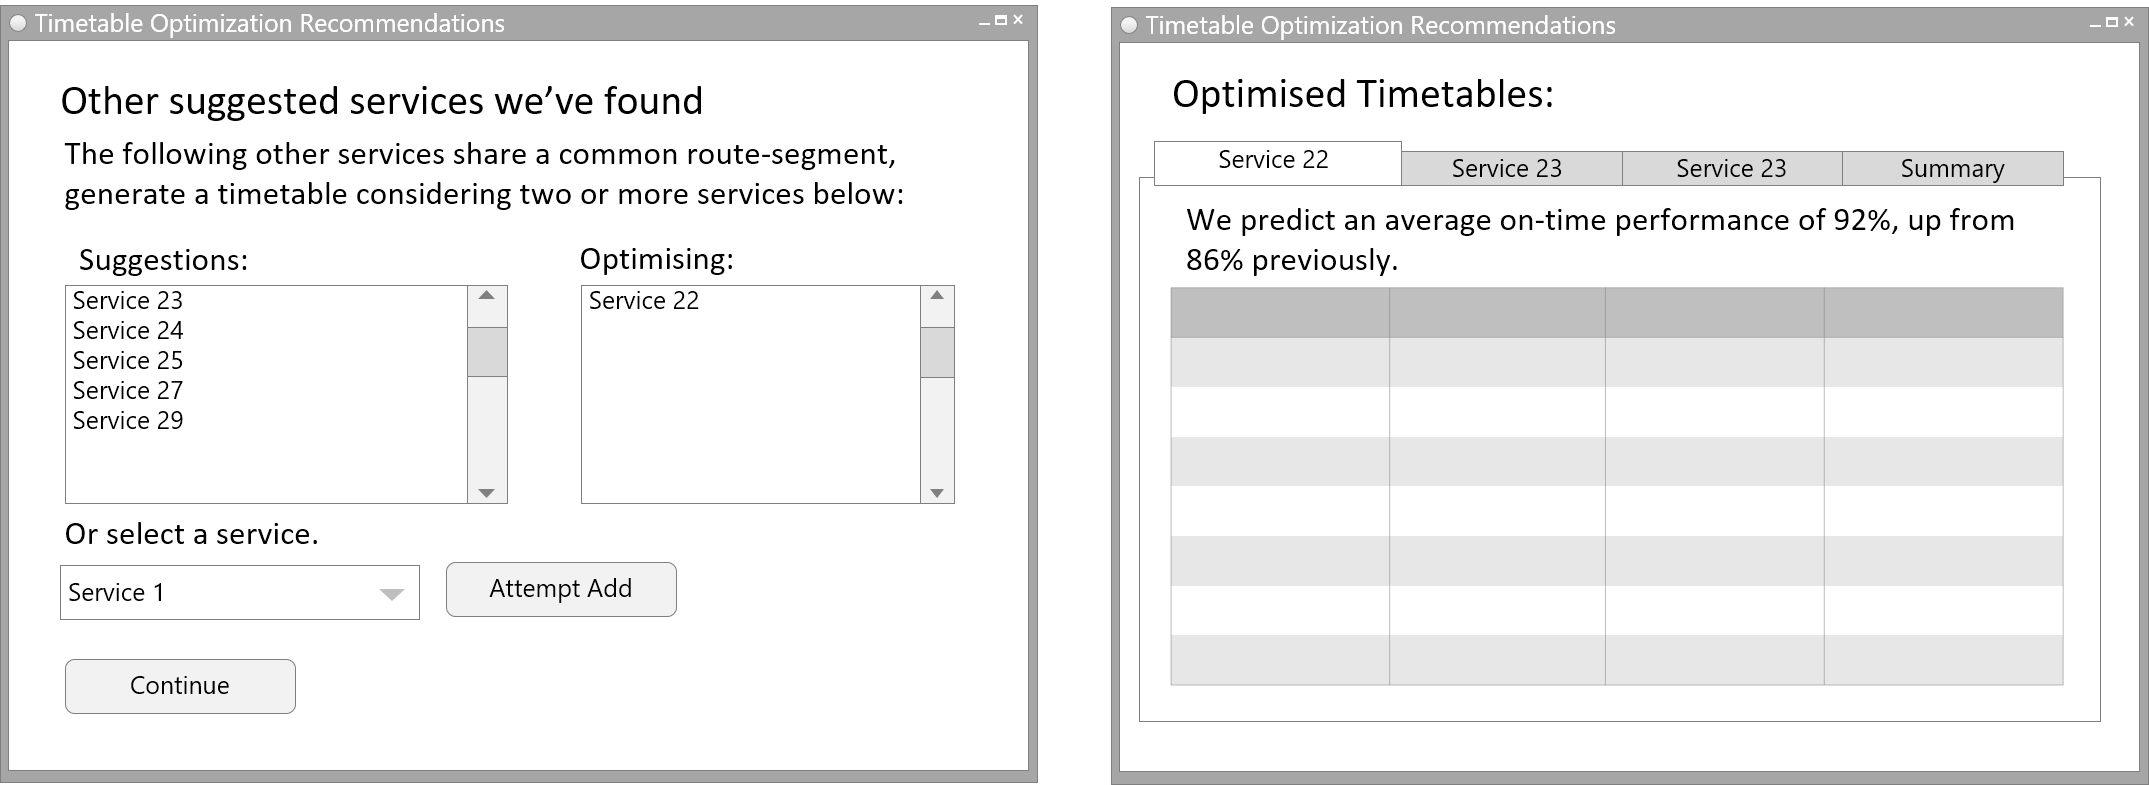
\includegraphics[height=110px]{images/GUI_2.png}
	\caption{GUI Design for Screens 4 to 5.}
	\label{fig:gui2}
\end{figure}

Finally, the actual optimised timetable for each service will be outputted, along with a set of estimated performance metrics. 

\par 
I will be implementing the GUI in an MVVM design pattern\cite{RN44}, as this allows for me to easily have ``separation of concerns'' between the user interface and the application logic. Which makes testing easier and allows for the GUI to be updated with ease in the future. In WPF this is achieved through the use of data-binding in the XAML and Visual Studios has several tools to assist me with this.


\subsection{Dataset}
For this project, I decided to use the Reading Buses Open Data API (RBOD-API), due to its exemplary level of data access, providing a year's worth of historical bus timetable data, information on their bus stops and services operated and one month of historical GPS data, which can all be queried, by vehicle, service, stop and date. 

\par
Transport for London, West Midlands Transport, the National Bus Open Data Portal and Transport API UK, all provide a range of public transport APIs either for free or at a low cost. Unfortunately, none of them provide historical data. While it is possible to request the data each day and make my own historical backlog of data, this would take several weeks to accumulate enough usable data and as such makes these impractical to use. All other bus operators in the UK are currently only providing a very limited set of public APIs, with the majority requiring authorization directly from the operator. Something I hoped to avoid, as this would have taken several weeks to organise and get access. 


\par
Reading Buses, however, does not provide Automatic Passenger Counter (APC) information, while they do record ticket sales; this data is not publicly accessible, nor do they record when passengers are alighting. Although, as I am not considering constraints of vehicle capacity I do not deem the lack of access to this data to be much of a hindrance. 


\subsubsection{Reading Buses Open Data API Library Design}
For the library, I planned on creating a .NET Standard 2.0 \CS \ Class Library, this is because .NET standard provides the greatest level of portability between .NET versions and operating systems. The library should interface with the following Reading Buses REST APIs: List of Bus Stops, List of Services, Line Patterns, Timetabled Journeys, Tracking History. While they also provide historical GPS data (and several live feeds), I do not need these for the project.


\par 
As the majority of the data provided by the API is in a proprietary format, as opposed to the standardised TransXChange format\cite{RN28}, I had to create a custom solution to parse and interface with the API for my project. I proposed a design, which has a main singleton controller, called ``operator'', which lets you get a list of bus services and stop locations. Once you have a Bus Stop or Bus Service object you can then query further data about it. Which should be more intuitive than creating a class per API feed.

\subsection{Data-Schema Design}

\par
While this project utilises the RBOD-API, I wish for it to be portable to use with any operator's API, particularly with the trend for bus open data APIs in recent years. While there are standardised ways for representing bus timetables and GPS data, I need for it to be formatted and processed in a useful way, so that it can be easily reasoned with. As such, I generated a data scheme, by creating a set of interfaces, from which a class will implement to provide the functionality for an operator's API.


\subsubsection{Bus Stop}

\begin{figure}[H]
	\centering
	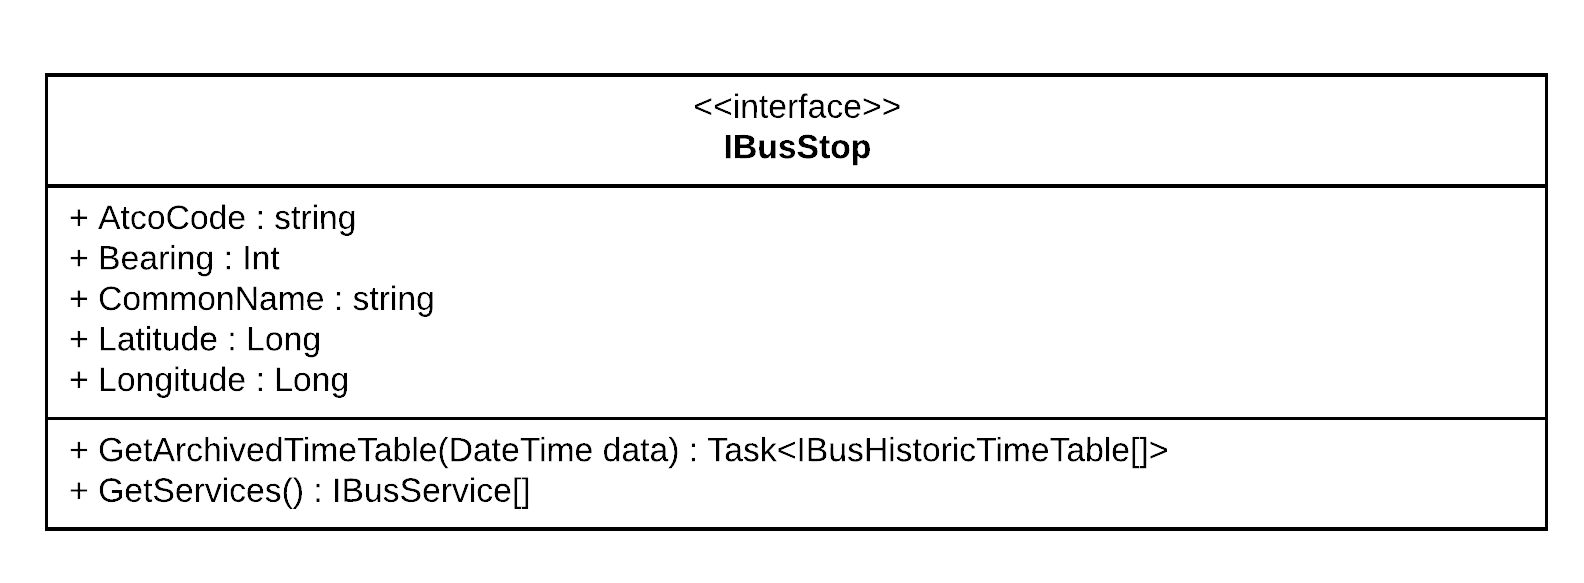
\includegraphics[width=300px]{images/CD_Stop.png}
	\caption{Bus Stop Data Class}
	\label{fig:busstopdata}
\end{figure}


Each bus stop has a NaPTAN ATCO Code, this is a unique alphanumeric string that can identify any bus stop in the UK. I stored the stop's geographical location as a longitude, latitude and bearing value. Finally, I stored the services which visit the stop and provide the ability to get the archived timetable record data at the stop by date.  


\subsubsection{Bus Service}
\begin{figure}[H]
	\centering
	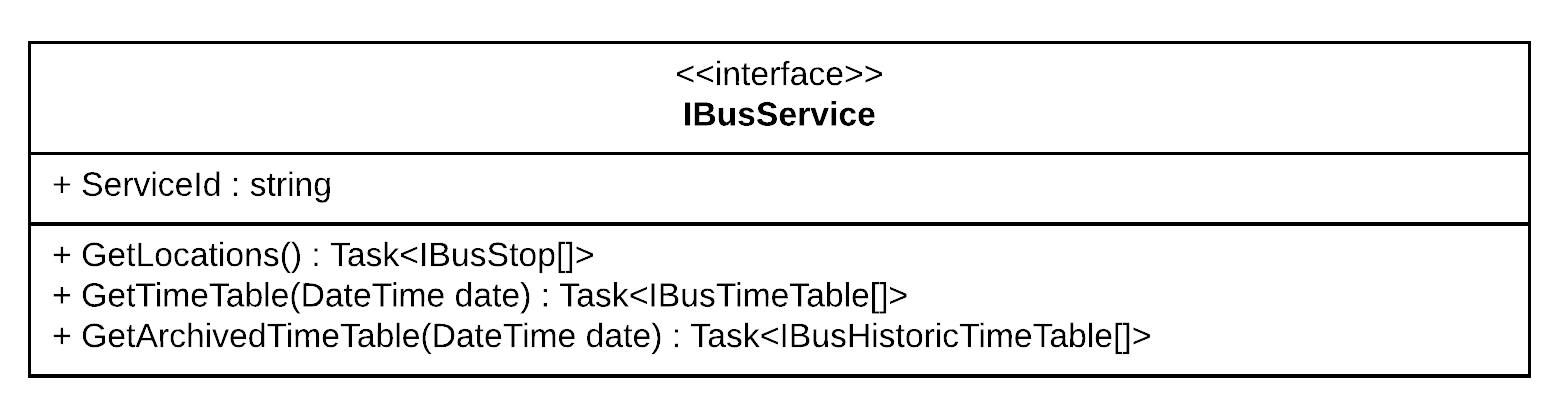
\includegraphics[width=300px]{images/CD_Service.png}
	\caption{Bus Service Data Class}
	\label{fig:busservicedata}
\end{figure}

Each bus service object has its own unique alphanumeric service ID and provides the ability to get a list of bus stops the service visits. Including the historical scheduled timetable and historical journey trip information, on a specific date.


\subsubsection{Timetable Record Representation}
\label{timetableRecord}

\begin{figure}[H]
	\centering
	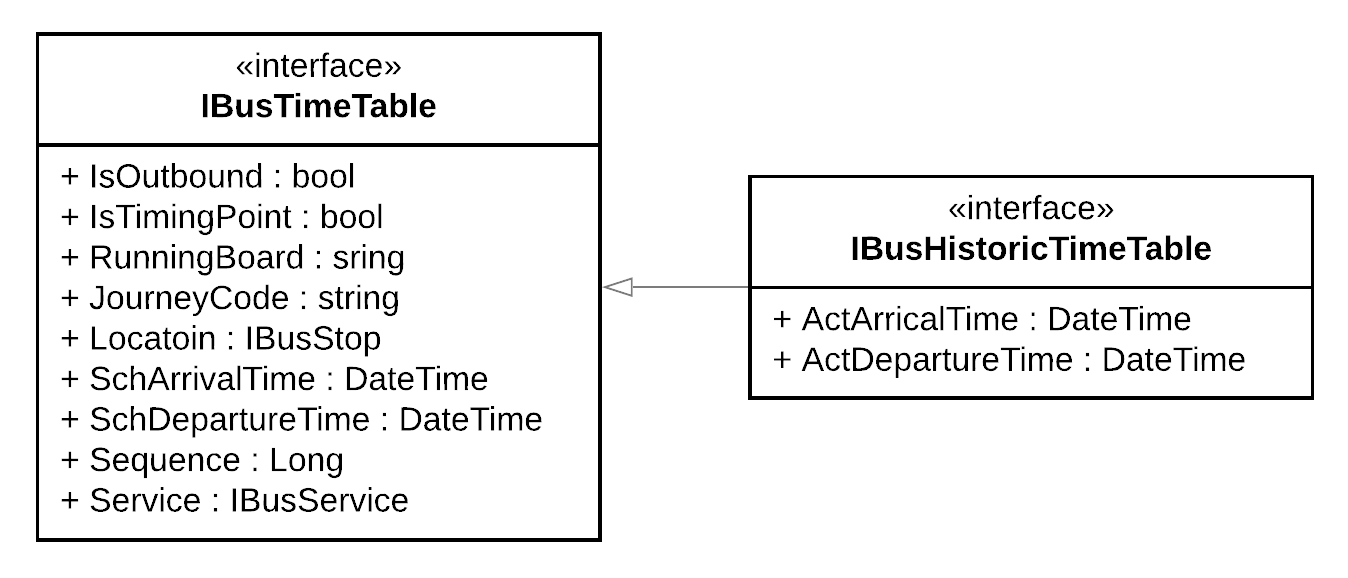
\includegraphics[width=300px]{images/CD_TimetableH.png}
	\caption{Bus Time Table and Historical Time Table Record Data Class}
	\label{fig:bustimetabledata}
\end{figure}


A timetable is represented as an array of ``records'', which are stored by the ``\texttt{IBusTimeTable}'' interface. A record is information about one single bus of a service stopping at one single stop, at one time. It contains the following key attributes:

\begin{itemize}
	\item The bus stop and service it pertains to.
	\item Scheduled Arrival and Scheduled Departure Time.
	\item Sequence Number - The index of the record in the journey.
	\item Journey Code - A unique identifier for the current journey, defined as one full sequence of inbound or outbound stops.  
	\item Running Board- An identifier that groups together journeys that are performed by the same drive in a shift.
	\item Is Timing Point- Used to identify if the stop is a timing point for this service record.
\end{itemize}

``\texttt{IBusHistoricTimeTable}'' further extends from this to add on Actual Arrival and Departure Times. 

\subsubsection{Importance and Relevance}
Therefore, I have produced concrete classes that implement from these interfaces for the RBOD-API. This is significant because each object might contain calls to several API feeds, for example, the \texttt{RbBusService} class calls upon the Line Patterns, Timetabled Journeys and Tracking History API. Compartmentalising several feeds into a single object is more intuitive to develop for and API independent. Moreover, it explicitly sets the requirements for what other API feeds must be able to provide if you were to implement a new bus operators API in the future. 

\par 
Within each of these concrete classes a caching solution is in place coupled with lazy evaluation to ensure performance is as good as possible. See section \ref{caching} for a detailed breakdown.



\subsection{Simulation Methods}
\label{simulation}

An important required ability is to be capable of simulating how a bus service would operate once changing the timetable, there are two main things I must consider:

\begin{itemize}
	\item  The estimated travel time between two stops at that specific time of day, as the traffic conditions change throughout the day travel times will not be consistent.
	\item  The required dwell time at a stop at a specific time of day, to allow for passengers to alight or board at a stop in time; this will change throughout the day as passenger demand changes. As Reading Buses does not provide APC information, this was needed to be estimated.
\end{itemize}

 

\subsubsection{Travel Time Estimation}
\par 

The time of day you wish to know an estimated travel time between two stops is referred to as the ``Target Time''; this can be either an arrival or departure time of the second or first stop respectively. Given a day of historical data from one service (that is known to travel between these two stops), I look at the travel times of the vehicles directly before and directly after the target time. With these two known travel times, I proportionally grow or shrink towards either of the two known times, based upon how close the time of the known journey is to the target time, generating a new estimated travel time.



\begin{gather}
	\label{proposedTime}
ProposedTravelTime = T_2 * \dfrac{D_2 - TargetTime}{D_2 - D_1} + T_1 * \dfrac{TargetTime - D_1}{D_2 - D_1} \\
AccuracyRating = \dfrac{1}{Min(TargetTime - D_1, D_2 - TargetTime)} 
	\label{proposedTimeAcr}
\end{gather}

\begin{align*}
	\text{where~$T_1$ is the Travel Time for the journey directly before our target} \\
	\text{$T_2$ is the Travel Time for the journey directly after our target.} \\
	\text{$D_1$ is the Departure Time for the journey directly before our target} \\
	\text{$D_2$ is the Departure Time for the journey directly after our target.}
\end{align*}

\par 
I repeat this process for every known service between the two stops and for every day worth of data, generating several new proposed estimated times, as highlighted in Figure \ref{fig:travelTimeDay}.

\begin{figure}[H]
	\centering
	
\includegraphics[width=300px]{images/travelTimeDay.png}
	\caption{One Day Travel Time Estimation Visualised}
	\label{fig:travelTimeDay}
\end{figure}


\par
Each time is given an associated accuracy rating, which will later be used as a weight. This accuracy rating is generated based upon the inverse of the smallest of the two differences from the target time to actual time. 

\par
For example, say we wanted to know how long it would take a bus to travel from Stop A to Stop B departing at 9:30AM. I will look at one single day of historical data from one service for this example. In the historical data a bus departed at 9:15AM, taking 2:22 and one at 9:50AM taking 3:06 to travel. 9:15AM is only 15min off of our target time of 9:30AM, compared to 20min of the second journey. As such, we weigh more towards the journey time taking 2:22 and have an accuracy weighting of 1/15. This process would be repeated for all services and all days of data.

\begin{figure}[H]
	\centering
	
\includegraphics[width=350px]{images/travelTime.png}
	\caption{One Day Travel Time Estimation Visualised}
	\label{fig:travelTime}
\end{figure}


\par 
Within the code, this is stored as an array of tuples of estimated time with an accuracy rating. The final estimated journey time is calculated by working out the weighted average of all estimated times against their accuracy rating, to make one final value. 


\begin{gather}
	EstimatedTravelTime = \dfrac{\sum^{Z}_{n=0} (ProposedTravelTimes_n * AccuracyRatings_n) }{\sum^{Z}_{n=0} AccuracyRatings_n}
\end{gather}


\begin{align*}
	\text{where~$ProposedTravelTimes$ is an array of estimated times of travel,} \\
	\textit{ generated from Formula \ref{proposedTime}.} \\
	\text{$AccuracyRatings$ is an array of assoicated accuracy ratings for the estimated time, } \\
	\textit{generated from Formula \ref{proposedTimeAcr}.} \\
	\text{$Z$ is the length of the WeightedTimes and AccuracyRatings Tuple Array.} \\
\end{align*}


\par 
This method would not necessarily work where there is a lack of frequent data records, you are predicting a time after or before the final or first historical journeys respectively, or where you are making significant timetable changes. Moreover, for high-frequency services you may get better accuracy by taking more than just the first two journeys on either side.

\par 
However, as one of my optimisation targets is to minimise large changes and I used any service that goes between the two stops as data points, I judged there was enough data to be a reliable approximation. 


\begin{algorithm}[H]
	\SetAlgoLined
	\KwIn{Target Time of Arrival or Departure, Services Between Stops, Start Stop A, End Stop B, Dates of Data}
	\KwResult{ An estimated theoretical journey time between two stops at a time of day specified. }
	
	
	ListOfProposedTimes $\gets \emptyset$ 

	\ForEach{ Service $\in$ Services}{%
		Data $\gets$  HistoricalTimeTableData(Dates)
	
		\ForEach{ Day $\in$ Data}{%
		
			Filtered  $\gets$ Records Between Stop A and Stop B $\in$ Day
		
			JourneyBefore $\gets$  JourneyJustBeforeTargetTime(Filtered )
			
			JourneyAfter $\gets$  JourneyJustAfterTargetTime(Filtered )
			
			
			(ProposedTime, AccuracyWeight) = GenerateWeightedAverage(JourneyBefore, JourneyAfter)
			
			ListOfProposedTimes.Add((ProposedTime, AccuracyWeight))
		}
	}

	\KwRet(WeightedAverage(ListOfProposedTimes))
	
	\caption{Estimating Travel Times At Different Times of Day}
\end{algorithm}


\subsubsection{Required Dwell Time Estimation}
\par
To calculate the historical dwell time, at a timing point stop, there are two situations to consider:
\begin{itemize}
	\item The bus arrives early at the stop - therefore,  we must assume that it will wait at the stop until it is scheduled to leave. So the time used will only be from the scheduled departure time to the actual departure time.
	\item The bus arrives late to the stop - therefore, the bus should have left as soon as it could have, in which case the actual arrival time and actual departure time can be used. 
\end{itemize}

\par
If the stop is not a timing point then the bus has no obligation to remain at it for longer than required, in which case we can simply use actual departure time minus actual arrival time. It is important to note, that a stop might be a timing point for one service, but not another, so data can be gathered from several services using both methods at the same stop.


\begin{algorithm}[H]
	\label{dwellAlgorihtm}
	\SetAlgoLined
	\KwIn{Timetable Record}
	\KwResult{ An estimated amount of time a vehicle dwelled at a stop. }


	\If{Is A Timming Point}{
		\If{Actual Arrival Time $\geq$ Scheduled Arrival Time}{
			\KwRet{Actual Departure Time - Actual Arrival Time}
		}	
				
		\If{Actual Departure Time - Scheduled Departure Time  $<$ 0}{
			\tcp{If a bus left earlier than it was allowed to, return zero. As it should not have done so.}
			\KwRet{0}
		}
		\KwRet{Actual Departure Time - Scheduled Arrival Time }
	}	
	
	\KwRet{Actual Departure Time - Actual Arrival Time}
	
	\caption{Calculating Dwell Time From Historical Data }
\end{algorithm}

If a bus departed earlier than it was scheduled to at a timing point, it should not have been allowed to and as such zero is returned instead, from testing this was a very infrequent occurrence and so does not pose much of a risk to the final average value.  

\par 
The obvious downside of situation one is passengers can be alighting and boarding during the time in which a bus arrives earlier than was scheduled to at a timing point stop. Hence, not being recorded and so not giving a true reflection of the needed dwell time. Furthermore, this assumes that all services are using similar vehicle designs (capacity, ticketing methods/machines and the number of doors), so the time to board and alight can be compared between services.

\par 
Similarly to the Travel Time Estimator, I requested the bus stop data for every day of interest. To speed up this process I implemented the option for ``Weak Stop'' data, this is where instead of querying the API specifically for historical stop data, the data is built from pre-existing cached historical services data. Filtering out the records that only pertain to the selected stop of interest and then combining all the services at the stop together. This data is already cached and is likely to return a similar result to what the API would have, but generating it is significantly quicker.


\par 
Likewise, the process iterates through every day of historical stop data, finding the record directly before and directly after the target time. Calculates the dwell time for both, and then performs a weighted average depending on the time deviation from the target time to produce a new proposed time. This proposed time is given an associated accuracy weighting, from the inverse of the minimum deviation from the target time. A single final estimated dwell time is then calculated from weighted averaging all proposed dwell times against their accuracy weighting.


\begin{algorithm}[H]
	\SetAlgoLined
	\KwIn{Target Time of Arrival, Bus Stop, Services At Stop, Dates of Data}
	\KwResult{ A estimated theoretical dwell time at a stop at a time of day specified. }
	
	
	ListOfProposedTimes $\gets \emptyset$ 
	
	Data $\gets$ GetStopData(Dates)
	
	\ForEach{ Day $\in$ Data}{%
				
		RecordBefore $\gets$  RecordJustBeforeTargetTime(Day)
		
		FirstDwell $\gets$ DwellCalculate(RecordBefore)
		
		RecordAfter $\gets$  RecordJustAfterTargetTime(Day)
		
		SecondDwell $\gets$ DwellCalculate(RecordAfter)
					
		(ProposedTime, AccuracyWeight) = GenerateWeightedAverage(FirstDwell, SecondDwell)
		
		ListOfProposedTimes.Add((ProposedTime, AccuracyWeight))
		
	}
	
	\KwRet(WeightedAverage(ListOfProposedTimes))
	
	\caption{Estimating Dwell Times At Different Stop and Times}
\end{algorithm}



\par 
Although, taking only the very first records on either side of the target time for high-frequency stops does not necessarily provide a true reflection of the dwell times. 

\par
For example, if the target time was 11:35AM, but bus bunching occurred on a day, and at 11:30AM a bus arrived, and dwelled for four minutes picking up a backlog of passengers, but then at 11:33AM a bus arrives and dwells only for 30 seconds. Then the 11:33AM bus would be the first record directly before our target time, falsely giving the impression of only a 30second required dwell time. 

\par 
Alternatively, you could take the ``$N$'' records directly before and after the target time and then apply the weighted distribution algorithm, which would produce a Gaussian distribution of weightings. However, having several days worth of data should even out any outliers, which is why I decided the added complexity was not justified. 

\par 

The total time for a bus to travel from one stop to another is therefore equal to \( Travel Time + Required Dwell Time\). 





\subsection{Considered Optimisation Strategies}
\label{strats}
Through my research on optimisation algorithms and related works, I identified the following promising types of algorithms I could have used for this project. As such I have briefly explained them and their positives and negatives below:

\subsubsection{Genetic Algorithm}
By far the most popular optimisation technique currently researched in the bus timetable optimisation area is the use of various Genetic Algorithms (GA). GAs are based upon the theory of natural selection by Charles Darwin \cite{RN35}. They start with multiple different solutions (known as chromosomes) to the problem which are evaluated to determine how good they each are; only the evaluation function has any domain knowledge. The best chromosomes are then selected to ``breed'' with each other, which then produce a new solution mixing the different properties (genes) of both solutions. This process is then repeated until some condition such as time or number of populations has been reached. The solutions are then evaluated to determine how good they are. The hypothesis is that by combining good solutions even better solutions are produced. Mutation can also occur, this is where a property of a chromosome is changed at random, doing this prevents premature convergence.

\par
GAs can work faster and use less memory than other optimisation algorithms. However, randomisation means that it is not optimal and can get stuck in a local maxima, it can also be very difficult to be able to represent the problem as a bit string or otherwise. As such, due to their complexity, I decided that this would have been overly difficult to implement given the time.  

\subsubsection{Integer Programming}
Another popular technique is Integer Programming (IP), this is where the problem is formulated as a mathematical representation, with an objective function to maximise and a set of linear constraints. This could further be advanced with Mixed-integer linear programming, where not all of the constraints must be integer. However, as IP is primarily used to represent the problem more as a mathematical model, I did not believe that this would be an appropriate solution as representing service cohesion would be particularly difficult mathematically. Moreover, while linear programming is easy to understand, I was more interested in learning an algorithmic approach.

\subsubsection{Local Searches}
Another possibility was the use of a local search algorithm, these are heuristic methods, which apply local changes to try and improve the current state and will do so until a time/attempt limit has elapsed, or a solution is deemed acceptable.

\paragraph{Hill-Climbing} is one form of local search optimisation. It starts with a solution to the problem, for example, the current timetable in place, and then tries to iteratively find a better solution through incremental changes \cite{RN36}. If the change produces a better solution then it is kept and another incremental change is made on top of this solution until no more improvements can be found. Hill-Climbing is a relatively simple, but popular, search algorithm in AI. The problem with Hill-Climbing search is that it can get stuck in a local optima inside of the search space where the best possible solution cannot be found. To get around this a new start location is used, the size of the neighbourhood to search is increased, or use one of the more advanced algorithms below.


\paragraph{Tabu-Search} (TS) is a form of meta-heuristic algorithm, proposed by Fred Glover in 1986, which tries to avoid entrapment in cycles by forbidding certain moves which have previously been visited \cite{RN35} \cite{RN37}. Tabu-Search can accept non-improving solutions deterministically so that it can escape from a local-optima and try to find better solutions further on. Tabu-Search, therefore, needs to keep track in memory of the states which have previously been visited to prevent re-visiting them. Tabu-Search can be considered an extension of Hill-Climbing to allow it to escape from local-optimas


\par 
However, when there is a very large search space, or if more attributes are being stored than truly needed to represent the changes between stages; it can take a very long time just to check if you have visited the state before. Moreover, it can be a very memory intensive search and you risk exhausting a device's memory if the tabu-list is not constructed carefully. Tabu-Search therefore often generate a generally good solution for optimisation problems. But Tabu list construction is problem specific and there is no guarantee of a globally optimal solution. 


\paragraph{Simulated Annealing} (SA) is motivated by the physical annealing process, it mimics when a material is heated and slowly cooled down into a uniform structure \cite{RN35}. SA keeps track of a ``temperature'', when it is high the algorithm can accept a solution that is worse than our current one with a greater frequency. This allows it to escape from local optimums early in the execution. The temperature will gradually cool and as it does the probability of accepting a solution worse than the current reduces, which allows for it to gradually focus on a specific part of the search space.

\par 
SA is different to Hill-climbing because it will select its next move at random and decides whether to accept it with an acceptance function; whereas Hill-climbing will always choose the best move from all those available in the neighbourhood. This means that the results are generally not reproducible, as randomness is introduced. It should also keep track of what has been the best solution so far, as the last solution is not necessarily going to be the best.



\section{Implementation}
The following section outlines, the work I have carried out and highlights the parts of particular technical complexity. Ordering is based upon the order in which it appears in the flow of the program.



\subsection{Identifying Timetable Patterns}
\label{timetablePatterens}
After the user has selected the service they wish to optimise for, an important preliminary stage was to work out at what different timetables operated during the time region of interest specified. So that the user could then select for which timetable they would like to optimise and  this then lets me know for which dates in the year I should request historical timetable data for. Unfortunately, the Reading Buses API does not provide a simple way of achieving this.


\par
So instead, for each day I checked does it match the timetable of another known timetable, if so add the date to the timetable, else it is a new timetable and so make a note of it. While this method is not overly efficient there is only ever going to be 365 days worth of data to check and as such $O(n^2)$ complexity should not be much of an issue. 

\par 
The number of comparisons of records can also be reduced by first checking if the number of records in each timetable is different or not. If they have a different number of records then we already know they cannot be the same and do not need to be checked.

\par 
Unfortunately, the data quality of the Reading Buses Scheduled Timetable API is poor for some services. With some reporting having a new timetable each day with very slight variances. As such, the actual implementation seen in the \texttt{TimeTableGroup} class is less strict and requires predominately that the cardinality of the two timetables is the same. 

\begin{figure}[H]
	\centering
	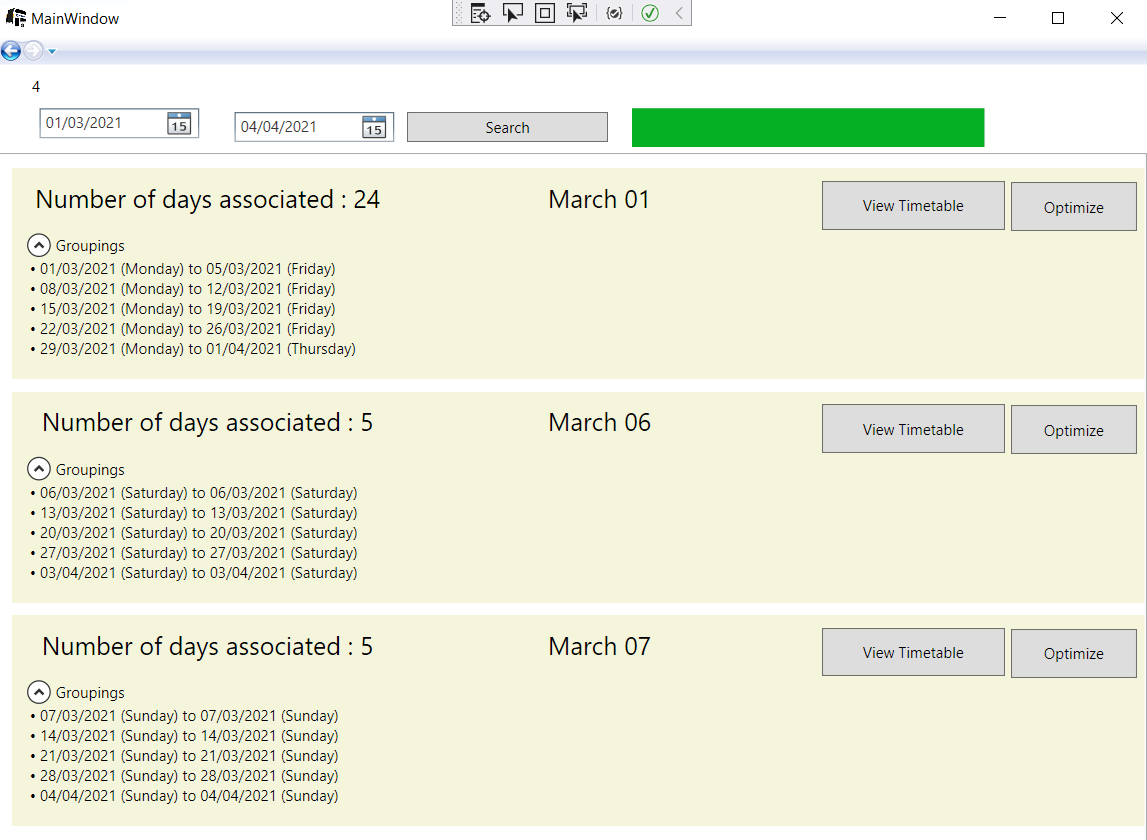
\includegraphics[width=300px]{images/grouping.png}
	\caption{Screenshot of Service 4 Identified Timetable Groupings}
	\label{fig:grouping}
\end{figure}

\par
Due to the sheer number of records in each timetable, it is very unlikely that two different timetables would have the exact same number. From testing, this has proven to be a successful implementation. As shown in Figure \ref{fig:grouping}, a different timetable was discovered for Monday to Friday, Saturday and Sunday. It also coped well with identifying new timetables on seasonal events, such as the period between Christmas to New Year.


\par 
Only the primary service has its timetable groupings identified, this is because if we were to look at the groupings of all services that are included in the search (due to having a shared route-segment), then we would be unlikely to find very much overlap of time periods within the group.

\par
For example, if we have Service ``A'' and Service ``B'', which both shared a common-route-segment, but Service A changed its timetable mid-way through a month, but Service B did not historically. Then it would make working out a single timetable for ``B'' that coheres with both of ``A''s very difficult. This could result in trying to find a balance for both but result with a timetable that works for neither of the two. This problem is compounded when you have several services, which might all have several different timetables throughout the period that the primary services timetable is consistent. 

\par 
To mitigate this, I made the assumption that the user will want all services that they are also optimising for, to have one single timetable for the same period of time as the primary service, regardless of what might have been historically the case. 

\subsection{Identifying Shared-Route Segments}
\label{sharedRoute}
After the user has selected the timetable group for which they would like to improve, I move onto identifying shared-route segments, such that I can meet one of my optimisation criteria of improving the cohesion between services in a shared-route segment.

\par
A shared-route segment is defined as ``N'' consecutive stops, shared by two or more services, where N is the minimum threshold number of consecutive stops required to be identified; three by default.  

\par 
The logic for identifying these shared-route-segments can be found within the \texttt{Route Analyser} namespace, with the \texttt{RouteSegmentFinder} identifying the segments and the \texttt{RouteSegment} class storing details about it. 

\par
I start by declaring a ``Long Term Memory'' list of route segments to be empty, then I iterate through every stop in the service, (re-)setting a ``Short Term Memory'' list of route segments to be empty at the start of every iteration.

\par
Next, I iterate through every service that is known to travel to the stop (ignoring itself.) I then check if in Long Term Memory there already exists a segment pertaining to the service of interest in this iteration. If not I simply start a new shared route segment (of length one) and add it to the Short Term Memory. If a route segment does already exist, then it must have been identified in a previous iteration and so have a segment length of one or more. 

\par 
I then add on the additional new stop (of the current iteration), remove the segment from the long term memory and add it to the short term memory list. After completing the inner-most for loop, going through every service, the remaining values stored within Long Term Memory are any Route Segments that have not been added onto in this iteration and so the service must have diverged from our primary service. 

\par 
The contents of long term memory is then iterated through, and if the route segment was greater than the threshold length, then it is added as a solution to the final route segment list. Short Term Memory now contains any route segment that was either newly created or added to in the current iteration. Therefore, long term memory is set to equal the short term memory, this means any service which was under the required length is discarded and the next iteration will have knowledge of continuing route segments.

\par 
This process is completed for all stops in the primary service until a final list of shared route segments can be found. The pseudocode in Algorithm \ref{alg:segmentCode} gives an overview of the logic:


\begin{algorithm}[H]
	\SetAlgoLined
	\label{alg:segmentCode}
	\KwIn{Primary Service, Route Segmenet Minimum Length Threshold}
	\KwResult{ A list of identified shared route segments. }
	
	
	RouteSegments  $\gets \emptyset$ 
	
	LongTermMemorySegments  $\gets \emptyset$ 
	
	
	\ForEach{ Stop $\in$ PrimaryService.GetListOfStops()}{%
		
		ShortTermMemorySegment  $\gets \emptyset$ 
		
		\ForEach{ Service $\in$ Stop.GetServiceAtStop()}{%
			
			\tcp{Do not include itself.}
			\If{Service = PrimaryService}
			{Continue}
			
			
			
			\tcp{If a non-finished segment already exists from the previous iteration}
			
			\uIf{``LongTermMemorySegments'' includes a segment already about ``Service''}{
				
				Segment  $\gets$ LongTermMemorySegments.Find(Service)
				
				Segment.AddStop(Stop)
				
				\tcp{Once updated remove out of long term memory and place into short term memory.}
				\tcp{This is so by the end of the iteration, the only values left in the LongTermMemory are segments found from the previous iteration that have no longer continued in this iteration.}
				
				LongTermMemorySegments.Remove(Segment)
				
				ShortTermMemorySegment.Add(Segment)
			}
			\tcp{Else it is a new segmenet not yet found.}
			\Else
			{
				NewSegment $\gets$ Make New Segment
				
				ShortTermMemorySegment.Add(NewSegment)		
			}
		}
		
		\tcp{If the segment no longer continued (it has ended) and if it is over the segment threshold length then add it to the solution.}
		
		AddToSolution(LongTermMemorySegments)
		
		\tcp{Then set LongTerm to be ShortTerm, so the next iteration knows what segments were found or continued from the previous iteration.}
		
		LongTermMemorySegments = ShortTermMemorySegment
		
	}
	
	AddToSolution(LongTermMemorySegments)
	
	\tcp{Validate the answer looking the other direction.}
	
	ValidateAnswer()
	
	\KwRet(RouteSegments)
	
	\caption{Identifying Shared Route Segments}
\end{algorithm}




\par
This final list is then validated, such that the converse for the secondary service in the route segment is true. For example, Service ``X'', might share 4 consecutive stops (1,2,3,4), with Service ``Y''. But Service ``Y'' does not necessarily also consecutively follow along the same route, it may make a divergence from ``X'', visit other stops (A, B) and then return back to it. As shown in Figure \ref{fig:divergance}.

\begin{figure}[H]
	\centering
	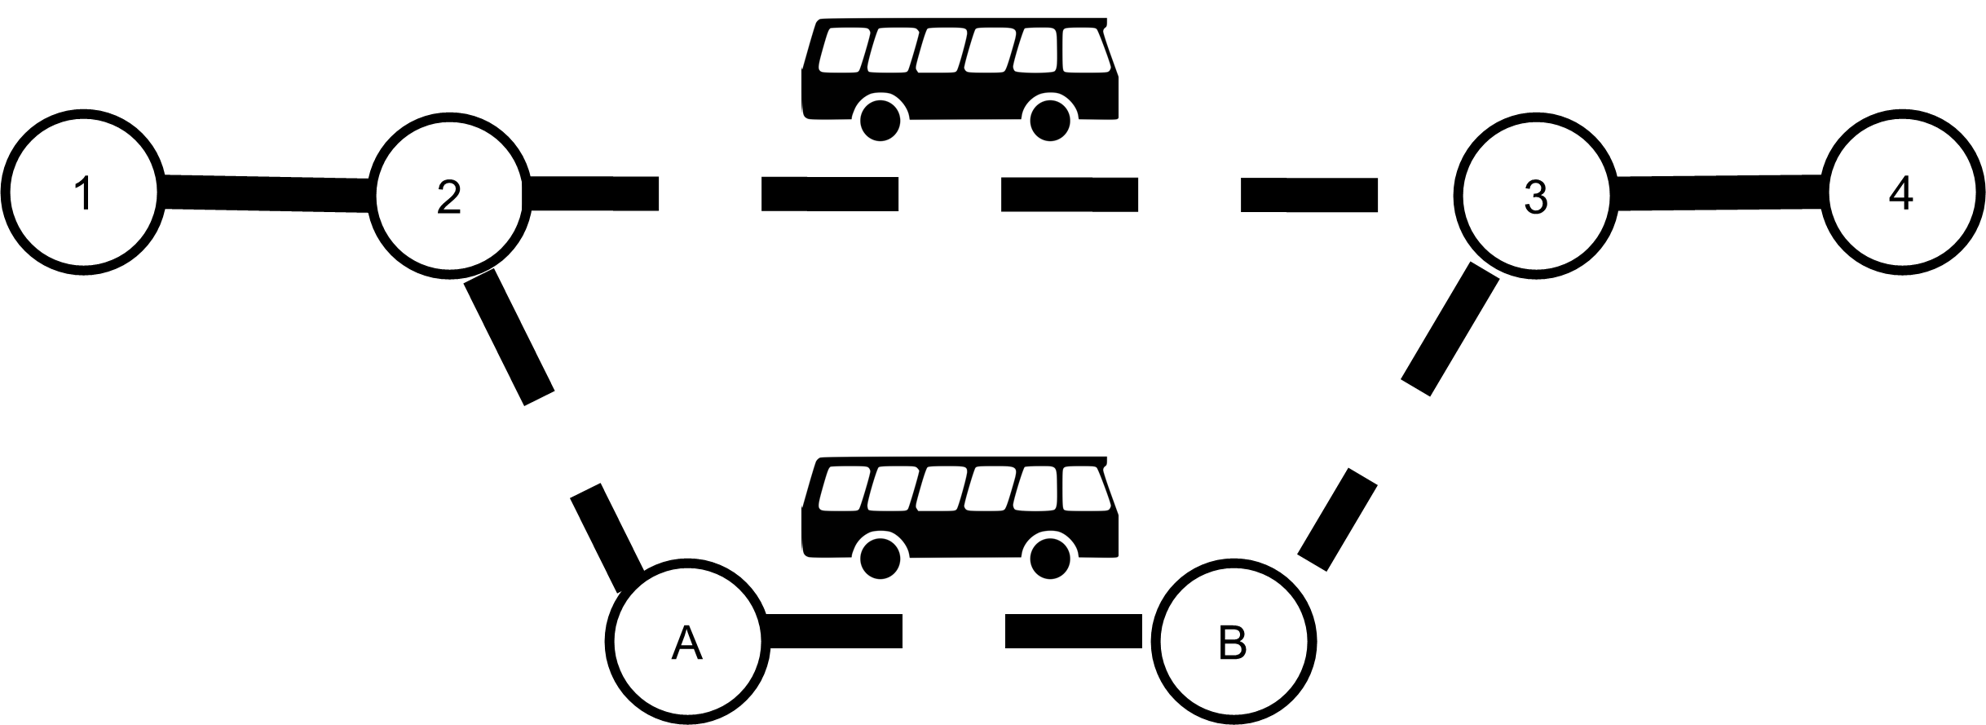
\includegraphics[width=300px]{images/divergance.png}
	\caption{Divergence Example For Validation}
	\label{fig:divergance}
\end{figure}


\par
In these instances, the route-segment should be considered invalid and removed, as this does not fit the formal definition of two services following the exact same consecutive stops. If one service takes longer than another then passengers will form a service preference, eliminating the need to form cohesion between them. 


\par
Unfortunately, there are locations where you have two stops directly next to each other, for example, ``Huntley and Palmers Stop 4'' and ``Huntley and Palmers Stop 5''. Which for the average passenger would be indistinguishable from each other. When waiting to board on any service travelling along a shared-route segment, they will quickly alternate between the two stops boarding upon whichever bus arrives first. 

\par 
As such, these stops should be considered perceptually the same and should be included in part of any shared-route-segment. At present they are not and can either break up a route-segment into two or cause a segment to be disregarded for falling under the minimum segment length. 

\par 
A possible method for future research that could have been used to mitigate this is to use the ``haversine'' formula \cite{RN43}, which would let me calculate the distance between the stops using their longitudinal and latitudinal points. I could then have made an assumption that they are perceptually the same if they have services travelling in the same direction and are close enough to each other. Another simpler solution would have been to look at the stops name and ignore any numerical value in the name, making ``Stop 4'' and ``Stop 5'' the same. This might not however work for all locations and careful evaluation would have been required.  

\par 
Neither methods were implemented, due to the rarity of the occurrences outweighing the time it would have taken to implement a solution.


\paragraph{Extending Out The Search}
I considered extending out the search, to include identifying shared route-segments of any other newly identified secondary services of the primary service. As if you are changing the timetable for a secondary service and it has its own shared-route-segments with other services, you are going to affect its cohesion and could worsen performance elsewhere in the network. 

\par 
However, I decided against doing this, because while Reading, has a predominately ``spider'' network design, where all services depart from some common location such as the city centre and spread outwards. There are a few services that span across this centre, an example being the popular Service 17, which travels from East to West Reading. In doing so, it will have shared route-segments with a very large proportion of services in Reading. 

\par 
Hence the search space can become increasingly very large, if you then continue to expand the search onwards you are likely to end up including all of the network in one. Something which I wished to avoid because it would be phenomenally computationally expensive and because of the aforementioned limitations of the timetable grouping algorithm, all services would have to have the same timetable throughout the same period of time. Meaning all services would have had to have changed their timetable at the same periods, something which is unrealistic and unrepresentative of the real world.



\subsection{Pre-Evaluator Checks}
After the user has selected the other services for which they would like to include in the search a pre-evaluator check starts. Here all data for the search is loaded into cache and performance metrics are generated for the original services timetables. Once all the required historical data is cached the actual search algorithm can begin.







\subsection{Search Algorithm}

The following section explains the search algorithm I selected, the stages of the search and how I have chosen to represent the problem.

\subsubsection{Chosen Search Optimisation Strategy}
I selected Tabu-Search as my primary optimisation strategy, as local-searches are relatively simple to create and conceptualise while generating generally good solutions in a short period of time. 

\par
Initially, I developed and tested out Hill-Climbing. But quickly identified that the search was frequently getting stuck in a local-optima and editing the same small subset of records repeatedly between iterations. 

\par 
In most instances, this was an issue with conflicting optimisation targets, where slack time would wish to push a timetable record in one direction and service cohesion another. Causing it to differ slightly each move, while making no real progress.

\par 
To prevent this from happening I built on top a tabu-list and implemented Tabu-Search to overcome Hill-Climbing repeatedly altering recently edited regions. Consequently, forcing it to alter other regions, with the hope that by making changes elsewhere it would indirectly resolve the issue, or at least give it time to explore elsewhere.


\par 
I considered Simulated Annealing over Tabu-Search, but decided it would not be as effective at preventing getting stuck in local-optimums and hence Tabu-Search was the more fitting solution to the problem.

\par 
Moreover, Tabu-Search is a popular and robust optimisation algorithm used in AI.  Although, there is very limited documented usage of Tabu-Search being used for bus timetable optimisation, this however gave me a unique area of research to explore and evaluate.


\par 
I have split the search into three key stages, which is explained below in order:


\begin{figure}[H]
	\centering
	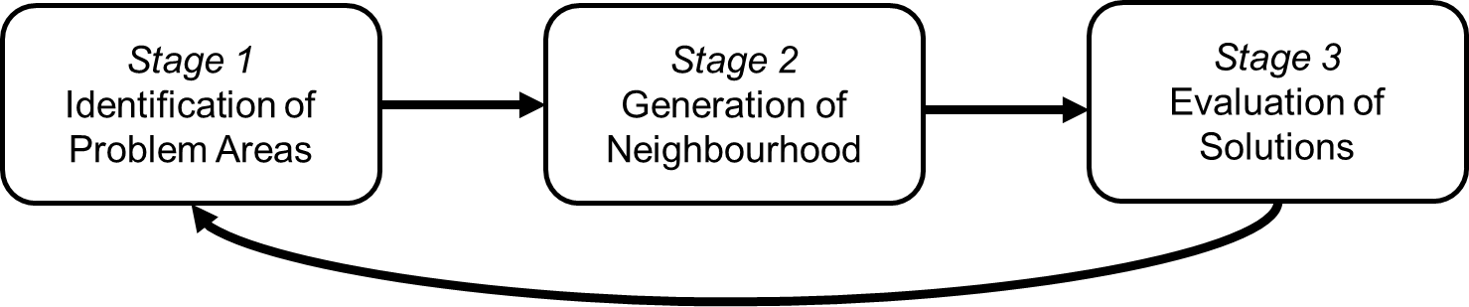
\includegraphics[width=250px]{images/searchCycle2.png}
	\caption{Search Stages}
	\label{fig:tabuSearch}
\end{figure}




\subsection{Stage 1 - Identification of Problem Areas,  Squeaky Wheel Optimisation}

Traditionally, Tabu-Search does not possess any domain-knowledge, other than in the objective function. However, due to the nature of the search space being so large, a more targeted approach was required in generating new solutions. As such, the first stage of the search is ``Identification of Problem Areas'', which was achieved using ``Squeaky Wheel Optimisation''(SWO) to help guide the search algorithm in the direction of a satisfactory solution. 

\par

\begin{figure}[H]
	\centering
	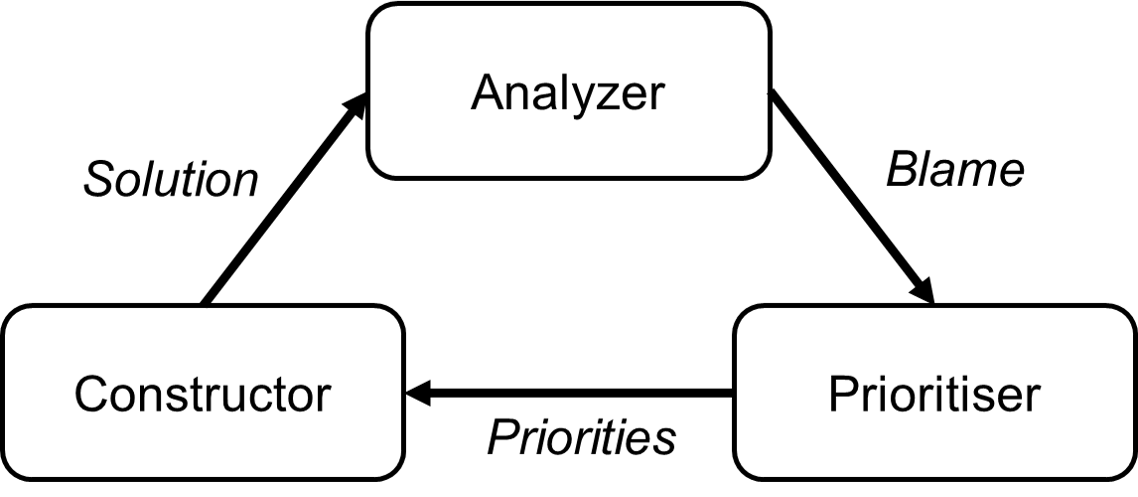
\includegraphics[width=250px]{images/swo.png}
	\caption{Squeaky Wheel Optimisation Cycle \cite{RN39}}
	\label{fig:swo}
\end{figure}

SWO can be summarised into three key stages, Construct, Analyse and Prioritise, as shown in Figure \ref{fig:swo}. In the first iteration, the pre-existing timetables are used as the first initial solution to the problem. As such analysis takes place first, the analyser looks at every timetable record and applies a numerical ``blame'' factor to it. The higher the blame factor the greater a problem the record is to the solution and the higher the priority is placed upon it to be altered. A blame value is given for each of the objective criteria of the problem, as explained below, with the sum of these values being the record's total overall blame.

\par
The prioritiser uses the blame values to generate a selection of moves, the greater the blame value the greater the change and more importance weighted to it. These moves generated form the neighbourhood solution space for the search algorithm. The aim is that by prioritising change to the most troublesome areas first, their blame values will decrease, causing new high-problem areas to rise; repeating the cycle to reduce the overall total blame and generating a better overall solution. However, due to how changes in the timetable propagate, there is no guarantee that the move will produce a better solution. 

\par 
The final stage is construction, this takes in the chosen move and generates the new solution. This solution is then fed back into the analyser and the cycles are repeated; guiding the direction of the search algorithm. David Joslin \textsl{et al}, described it as being useful ``to think of SWO as searching two coupled spaces'', the solution space and the ``priority space'' \cite{RN39}. Changes to the solution space will indirectly alter the prioritisation space and vice-versa, usually to a great effect. This is particularly true for bus timetables, where moving one record, causes a propagation of changes around it. 


\par 
For each of the optimisation targets, an objective function is created to evaluate it, this produces a numerical value that represents how well it meets this target. Objective functions can also be commonly referred to as cost and evaluation functions. However, due to these functions pertaining to SWO a common term used is ``blame''\cite{RN39} and henceforth I describe the ``score'' of the objective function as the blame value.


\subsubsection{Solution Representation}

A solution to the problem is abstractly just a set of new timetables for every service that we are optimising for. As mentioned previously in Section \ref{timetableRecord} a timetable is stored as an array of records. Although, these records also now need to contain logic and information about their blame weights for SWO. So a new `\texttt{BlamedBusTimeTableRecords}'' class is made that implements from ``\texttt{IBusTimeTable}'' and stores these blame values, both raw and normalised within the timetable.

\par 
Internally a solution is represented in the class ``\texttt{Solution}'', which provides a wrapper for a Dictionary where IBusService is the key and an array of BlamedBusTimeTableRecords is the value/timetable for the associated service. A dictionary allows the timetables to be grouped by service and provides a quick and efficient way to lookup their associated timetable. 

\texttt{Dictionary<IBusService, BlamedBusTimeTable[]> BusTimeTables}


\subsubsection{Slack-Time Objective Function}
\label{STOE}
One of the objective functions was to alter slack-time in the timetable, this was expanded to also include journey times and involves looking at the theoretically expected travel times and required dwell times to evaluate if the timings are ideal. The slack-time evaluator generates a blame-value based upon how many total minutes of difference there is between the scheduled arrival and departure times and the theoretical expected time; this value can be used to generate the target new arrival and departure time. For more information on the process of generating expected travel and dwell times see section \ref{simulation}.


 
\begin{gather}
	\label{slackBlame}
	SlackBlame_x = (ExpDeparture_x - SchDeparture_x) + (ExpArrival_x - SchArrival_X) 
\end{gather}
\begin{align*}
	\text{where~$Sch$ is currently scheduled value.} \\
	\text{$Exp$ is expected value, generated from simulation methods detailed in section \ref{simulation}} \\
	\text{$x$ is the array index.} 
\end{align*}


\par 
It can be thought of as how likely the bus is to be able to achieve the current timetable solution, given dwell and travel times. The higher the absolute value the less likely it will be able to achieve it.

\par 
The Slack-Time Objective Evaluator (STOE), can evaluate services independently from each other and so takes in each services timetable concurrently. This is important to note, because between iterations if the move does not alter the specific service, then the blame values will remain consistent and do not need to be re-evaluated (apart from being re-normalised). Which significantly increases the speed of subsequent iterations after the first.


\paragraph{Running Board ID} 

A services timetable is grouped by the records ``Running Board ID'', this is a numerical value that is used to indicate records that should be performed by the same driver during a shift. This has two main benefits, firstly, all records of the same running board are performed by the same driver and the same vehicle. This provides an easy way to identify which journey follows on after the next. 

\par
Which is needed when propagating changes and ensuring enough vehicles are available. For example, say the final record (at the last stop) of journey code 3 was increased by 10 min. But journey code 7 was scheduled to use the vehicle coming off of journey 3, then the start time of that journey must be later than the end time of the previous journey. If not, it too should be pushed backwards. With high-frequency services, the number of vehicles assigned to it varies throughout the day and journey-codes alone cannot be used to identify which vehicle comes off of one journey to start another. 

\par 
While there are other ways of working out which journeys follow on from another, such as looking at the vehicle registrations of historical data or making assumptions based upon the start and end times of journeys. Neither is as simplistic and definitive as using the running board ID.

\par 
The second benefit is, running boards are never likely to be longer than four to five hours, this naturally splits up the timetable into manageable chunks and restricts the maximum amount of propagation possible. That while not a true reflection of the real world, reduces the search space and improves the speed of the program, as there is less to compute. 


\par
The drawback is that my current implementation does not consider where a vehicle switches between different services. For example, in Reading, the vehicle operating service 22, becomes service 25 after completing every journey. While possible to account for this situation, I deemed it an infrequent enough occurrence not to consider given the time constraints.


\subsubsection{Service Cohesion Objective Function}
\label{SCOE}
The second objective function was improving service cohesion between services that share a common-route segment. Unlike the STOE, the Service Cohesion Objective Evaluator (SCOE) must re-calculate all blame values every iteration as any change, will affect the cohesion between all other services.

\par 
The SCOE can be considered as a measurement of how congested the stop is. The higher the absolute value the more congested it is at that time of day.


\par 
This SCOE works by iterating through all stops that are part of a known route-segment and then collecting all timetable records in the solution that pertain to the stop and are from a service in the route-segment. This can be thought of as getting an individual ``stops timetable'' and filtering it to only included service records of interest in the route-segment.


\par 
Next, these records are grouped into hourly blocks based upon the time that they arrive. Before iterating through each record in the hourly grouping and dividing the hour by the number of arrivals scheduled, to get the theoretical perfect spacing.

\par 
For example, say Stop A is part of a known route segment, containing services A, B and C, the timetable records for all these services that pertain to Stop A would be found and then grouped into hourly blocks. Say, between the time of 9 AM to 10 AM there are three buses arriving (and hence three timetable records), we would ideally have these three buses 20min apart from each other, at 9:00, 9:20 and 9:40 respectively; this would become the target times array.

\par 
Using the target times array I iterate through all current solution records in the group and mark down the time difference in minutes from the currently scheduled time to the associated target time. I work out the average difference amount and then calculate the difference each record is off of the average and make this the blame value, as shown in Formula \ref{cohesionBlame}.

\par 
This process is repeated for all hourly blocks throughout the stops timetable where there are at least two buses scheduled within and for all stops known to be a part of a route segment. As if there is only one service during an hour period there is no other service to cohere with.  
 
 
\begin{gather}
	\label{cohesionBlame}
	CohesionBlame_x = AverageDifference - (T_x  - R_x) 
\end{gather}

\begin{align*}
	\text{where~$T$ is the target record time array.} \\
	\text{$R$ is the scheduled record time array.} \\
	\text{$x$ is the array index.} 
\end{align*}


\par 
These values are then filtered and normalised, any stop which was not a part of a route-segment (so does not have a cohesion blame value),  is simply given the average blame value. This is so a blame value of zero does not weigh and skew the total blame value of the record, used to identify how much an issue it is.


This solution however has some shortfalls, the first being that this makes no account for the number of services that continue to share the route-segment at the next and subsequent stops. For example, between ``Stop A'' to ``Stop E'' you might have four services that share the same route-segment, and as such have a very short time difference between the target times. 

\par 
However, two of these services could diverge off, leaving the remainder of the route-segment with only two services. Hence, the target time difference would now be much greater, creating unrealistic targets without a service having significant wasted slack time. Which would then worsen the blame of our first objective. 


\par 
Keeping track of how the routes of the services changes and how best they should be scheduled proves a very complex problem. A similar problem with bus bunching has been discussed at length by Jan-Dirk Schmöcker \textsl{et al}, who considers how the head-way times affect passenger levels and subsequently boarding and alighting times; modelling this with a mathematical model dependant on whether a vehicle can overtake another or not\cite{RN40}.


\par 
I attempted to partially mitigate this issue, by using a more rudimentary solution of working out the difference from the average difference, such that if several records are being negatively affected by a change only those most affected are ``blamed''.


\par 
Another downside of this solution is that it does not account for the number of services per hour changing mid-way through the hour. This solution only works if the head-way frequency changes on the hour. This could have been mitigated by grouping into shorter time-periods, but you would need to vary the grouping period dependent upon the frequency of the services in the shared-segment. 

\par 
Finally, during some points in the day you may wish to explicitly have clusters of arriving buses, for example, outside a school at the start and home time. Moreover, a bus operator might deliberately decide to make one service arrive shortly after another if they anticipate passengers wanting to switch between them. As such, all records in the service would receive an unusually high weighting. Therefore, it does not necessarily reflect all real-world requirements. 


\par 
An alternative solution considered was calculating the difference between subsequent arrivals at a stop and then calculating the difference of that difference. However, this still suffers many of the aforementioned shortcomings of the current solution, while also only applying a high blame value onto the first record after a frequency change. Resulting in only a small handful of records, receiving blame values and moving each iteration; rather than considering moving several records at once.

\par 
Deciding upon the perfect times for maximum cohesion requires a lot of complex consideration of the route network design and intrinsic outside system knowledge, such as school times and locations for where bus bunching might be preferred. This however proposes an interesting area for future work.


\subsubsection{Change Tracking Objective Function}

The amount of change is simply tracked in each move, by working out the number of absolute minutes of difference made during the move. If the blame value is very high less preference is placed onto the move.



\subsubsection{Blame Normalisation}

\par
Once generated the blame values need to be normalised so that the blame values are comparable between different objective function blame types. I considered two methods of standardisation, the first:

\paragraph{Z-Score}

This is the value, minus the mean value of the set, divided by the standard deviation, as shown in Formula \ref{zscore}

\begin{gather}
	\label{zscore}
	\dfrac{value - \mu }{\sigma}
\end{gather}

Z-Score is not susceptible to any outlier data, but it cannot guarantee that the outputs will all be on the same scale. Which makes comparing blame value types less reliable. 

\paragraph{Min-Max Scaling}


\begin{gather}
\dfrac{value - min }{max - min}
\end{gather}
This is the value, minus the minimum value in the set divided by the range, it guarantees that all outputs will be in the range of 0 to 1 inclusive. This is useful as it allows for a better comparison of different blame values. However, any outliers in the data can skew the normalised values.

\par 
Therefore, I decided to use Min-Max Scaling, with a filter to remove any erroneous data. The filter simply drops the top and bottom 5 percentile of non-standardised weights; as this proved to be sufficient to remove most major outliers in testing. Then replacing their normalised blame with the average normalised value, so as to neither negatively nor positively impact their outcome. 




\subsection{Stage 2 - Generation of Neighbourhood Solutions}
Once the set of timetables have all been ``blamed'' by SWO, a set of possible moves and hence new solutions need to be generated.



\subsubsection{Move Representation}

A move is represented in the ``\texttt{Move}'' class, a move in the search algorithm will only ever alter one service's timetable at a time. Each move has a ``target record'', this is a specific timetable record identified as being troublesome and is being moved. A timetable record can be thought of as information about one bus visiting one stop at one time.

\par 
The target record is moved based upon the blame value suggestions, once the target record has been moved, the records around it also need to be moved (known as ``schedule repair'') to propagate the changes.

\par 
A move contains the new timetable for the altered service after the move has been applied with repair, along with several other properties such as, what records have actually been altered and how much so. As a move only ever moves one service at a time, the rest of the initial solution can be considered unchanged. 

\subsubsection{Schedule Repair}

When a target record has been moved the surrounding records must also be moved, for example, at ``Bus Stop B'', the service was originally scheduled to depart at 11:00 AM and arrive at the next stop, ``Stop C'', at 11:02 AM. But we now alter it so the bus departs Stop B at 11:05 AM, making it impossible to be able to arrive at Stop C on time ever if it remains at 11:02 AM. 


\par 
I can use the journey time and dwell time estimator, as explained in section \ref{simulation}, to generate a new time for Stop C, given a new departure time from the previous stop. The problem is, that by changing Stop C, we would then need to change the subsequent stop and continue this process onwards repairing the timetable until the end of the running board. Likewise, we would need to do similar for the stops before Stop B, to ensure the timing remains feasible or where the target record is moved backwards. Given the new time of day, passenger demand levels and traffic conditions change, affecting both dwell and journey times respectively.  


\par 
This poses two problems, the first being one of the optimisation targets was to minimise the total change, this is because a large number of changes makes predicting the real-world performance more challenging and uncertain. 

\par
The second is that this would significantly increase the computational cost of generating a brand new travel and dwell time for every record every iteration. Moreover, the journey time and dwell time simulator do not possess any domain knowledge. This means that by allowing them to change every record they can worsen the solution and override previous moves with every iteration. It would also require a more complex tabu-list implementation, to understand which of the records in the service are considered ``tabu''; further increasing the problem complexity.   

\par 
However, as I made the assumption that the initial solution (the currently scheduled timetable) is a feasible solution and I made only small changes to the target record, I did not necessarily need to propagate indefinitely, as the change could be ``absorbed'' gradually throughout the timetable. Due to the uncertainty of the real-world a scheduled timetable is never likely to be more precise than to the nearest 30 seconds, within this range is where journey times could return back to their original schedule. As such, I proposed a solution termed ``drop off'', where a random number is selected between 20 and 45. This is then the number of minutes added onto target records scheduled arrival time and becomes the ``drop off time''. 


\par 
The journey and dwell time estimator then produces an array of propagated timetable records up to the drop-off time. This propagated array is one where subsequent records rely upon the previous records changes suggested by the dwell and journey time estimator. Each of these propagated records is iterated over with the current solutions schedule and a weighted average is made between the two, dependent upon how close to the drop off time it is. This means that as the records get nearer towards the drop-off time they will slowly diverge back towards the originally planned schedule. 

\par 
This allows for a local region of repair to take place, without the whole solution being edited by one single move. Due to the target record change being so small and the propagation drop-off happening over several minutes I did not envisage any significantly infeasible times. However, if the propagation did produce unrealistic results then a subsequent iteration of the search would identify this and provide a fix. 



\subsubsection{Solution Neighbourhood Representation}

The neighbourhood solution is represented as an array of potential moves, the moves are generated by selecting the top ``N'' number of highest blame records across the current solution; where N is the size of the neighbourhood. Using each record as the ``target record'' and then performing schedule repair onto it, to generate a final potential move.

\par 
All services not detailed in the move can be assumed to have remained the same from the current solution and so are not stored within the neighbourhood to prevent the repetition of data and reduce memory consumption. 


\par 
By selecting the top N highest blamed records you target the most problematic areas with the hope that you fix these troublesome areas and improve the solution, but due to how timetables propagate and the cohesion between them, there is no guarantee this will produce the best moves.



\subsubsection{Probabilistic Tabu Search and Candidate List}

Traditionally, Tabu-Search involves evaluating every solution within the neighbourhood, however, if the neighbourhood is very large, the solution space very big and/or the objective function is computationally expensive to calculate, such as our problem. Then it can be a very time and resource-intensive procedure to evaluate all possible moves. 

\par 
As such I deployed the use of probabilistic Tabu-Search, this is where a random subset of the neighbourhood is selected, to form a candidate list and only this subset is then evaluated. This has the obvious benefit that you reduce down the search space, with every solution no longer being considered. But also has the added benefit of adding in diversification. By adding in an element of randomness, no single iteration will ever be the same and moves that might otherwise not have been selected, may become the best of the sub-set allowing for an otherwise unexplored region to be explored. 

\par
Although, as Fred Glover said, it is important to remember that  ``candidate list strategy should not be measured in terms of the reduction of the computational effort in a single iteration. Instead, a preferable measure of performance for a given candidate list is the quality of the best solution found given a specified amount of computer time''\cite{RN37}. This is because while it might become quicker to perform a single iteration, you might need to perform several more iterations to find a solution of equal quality, which could end up taking longer than the original search. This is particularly true for a pure probabilistic method, where the sub-set is chosen at random.

\par 
Therefore, my probabilistic method also takes its inspiration from a more complex candidate list generation method ``Successive Filter Strategy'' (SFS) to mitigate the risk of selecting poor moves. SFS, is where you break down a move into its ``component operations''\cite{RN37}, and then take the best ``N'' moves for each component group. This bears a resemblance to the individual blame values for a record generated during Squeaky Wheel Optimisation. SWO gives a greater knowledge of the neighbourhood ``terrain''. 

\par
While traditionally in Tabu-Search the terrain is defined by the objective function score, with SWO I have a more complex representation, where separate blame values are given for each optimisation target; which lets me know what are the most troublesome areas. Thereby, while targeting these troublesome areas does not necessarily guarantee the best solution, there is a greater probability it will, as such I can estimate the order of my neighbourhood.

\par 
Hence, similarly to SFS, I can from this order, probabilistically make a candidate list from the top ``N'' percentile of moves, growing ``N'' as required if moves are tabu and the cardinality of the candidate list is too small. This means it is not a purely random selection and I am more likely to be randomly selecting a good move over a bad.

\subsubsection{Tabu-List Representation}

To keep track of what are tabu-moves, I simply set all records within the drop-off region (including the target record) of the accepted move as tabu. These are blocked off in short-term memory for a customisable tabu-tenure length. While simplistic in design it helps ensure the search algorithm does not get stuck in a local-minima. Particularly, where the service cohesion and slack time objectives might be wanting the record to be moved in opposite directions. By blocking the record from being able to move in either direction for a set number of iterations after being changed, provides the opportunity for elsewhere in the solution to be altered, which may indirectly resolve the issue.

\par 
Hence, preventing getting stuck moving a small sub-set of records backwards and forwards in time. This is particularly important with timetables, where there is a continuous range of possible times, making it difficult to concern which solutions are different enough to be considered a ``new'' move. It is for this reason, I decided to tabu any move onto the records in question, as opposed to looking at the specifics of the amount of change and direction.


\par 
As the move does not need to be evaluated to establish if it is tabu or not, it can be removed from the neighbourhood of solutions at this stage, before evaluation has taken place.




\subsubsection{Intensification}

One area of future research I could explore is ``intensification'', this is where if the search has made several non-improving moves, it will return back to the last known ``best move'' and explore one of the other moves it could have made at that point. The main idea is to search more thoroughly in an area of the search space that was promising to try and find an even better solution. 

\par 
However, as the search rarely made non-improving moves, I decided that this was not required from testing given the time limits in place.



\subsection{Stage 3 - Evaluation of Solutions}

Once the search has generated the neighbourhood of solutions, each solution needs to be evaluated and the best solution selected.


\subsubsection{Solution Objective Function Score}
To evaluate the solutions, SWO is applied onto all of the new solutions and the solutions objective score value is then generated by the sum of the absolute value of the un-normalised blame values of all records. The lower this value the better the solution, with zero being a theoretically ``perfect'' timetable.  


\begin{gather}
	Solution Objective Score  = \sum^{Z}_{n=0} (Abs(Raw Slack Blame_n) + Abs(Raw Cohesion Blame_n))
\end{gather}


\begin{align*}
	\text{where~$n$ is the index in the array of timetable records.} \\
	\text{$Z$ is the length of the array of all timetable records in the solution. } \\
	\text{$Raw Slack Blame$ is the non-normalised slack blame value.} \\
	\text{$Raw Cohesion Blame$ is the non-normalised cohesion blame value.} \\
\end{align*}

All solutions will always have the same number of records and the raw blame value is the number of minutes of difference between the current time of the record and the time it wants to be at. Therefore, the sum of these values is the total number of minutes of difference between what it thinks is ``perfect'' and the solution. Hence, whichever solution has the lowest score is the best solution of the set and is then selected for the next iteration.

\par 
After performing stage three, the subsequent iteration stage ones can be significantly faster because the SWO blame values will already have been re-generated for the solution in this stage to calculate its overall solution score; thus speeding up the overall speed of the search.



\subsubsection{Termination Criteria}

Normally the termination criteria of Tabu-Search is defined as a fixed number of iterations, time, number of iterations without improvement or when the objective function meets some threshold value \cite{RN35}.

\par 
I considered limiting it based on time. But realised that the time for one single iteration would vary greatly based upon the number of services and days of data selected; meaning the number of iterations and the quality of the answer would vary drastically.

\par 
I also considered termination based upon a threshold Solution objective function score, however, due to the nature of how this value is calculated, it is dependent upon that specific search. The objective function value from one search cannot be compared against another search, as the number of services selected (and the number of total timetable records within each service) will affect what is considered a ``good'' score. 

\par 
As such, because time and threshold objective scores do not provide a standardised method for specifying the quality of a solution I chose to use iteration limit. There is no guarantee that ``N'' iterations of one search will produce the exact same quality as ``N'' iterations of another search, due to the random nature within the search itself. But iteration count provides a more reliable measure of comparison and as such, I have chosen to use it.

\par 
I could have considered terminating after a fixed number of iterations without improvements found, but choosing this value is non-trivial as it is not clear how many iterations must pass before an improved solution is unlikely to be found. Although, I did add in an ``End Early'' button and a visual counter to show if the search is improving or not and if so for how many moves it has been un-improving for. To aid the user with the decision of terminating the search early.

\par 
Throughout iterations the evaluator keeps track of what the best solution was and the current solution, this is because the best solution might not have been the final most current solution. Only the best solution is returned and displayed to the user.


\subsection{Multi-Tier Data Caching}
\label{caching}


\begin{figure}[H]
	\centering
	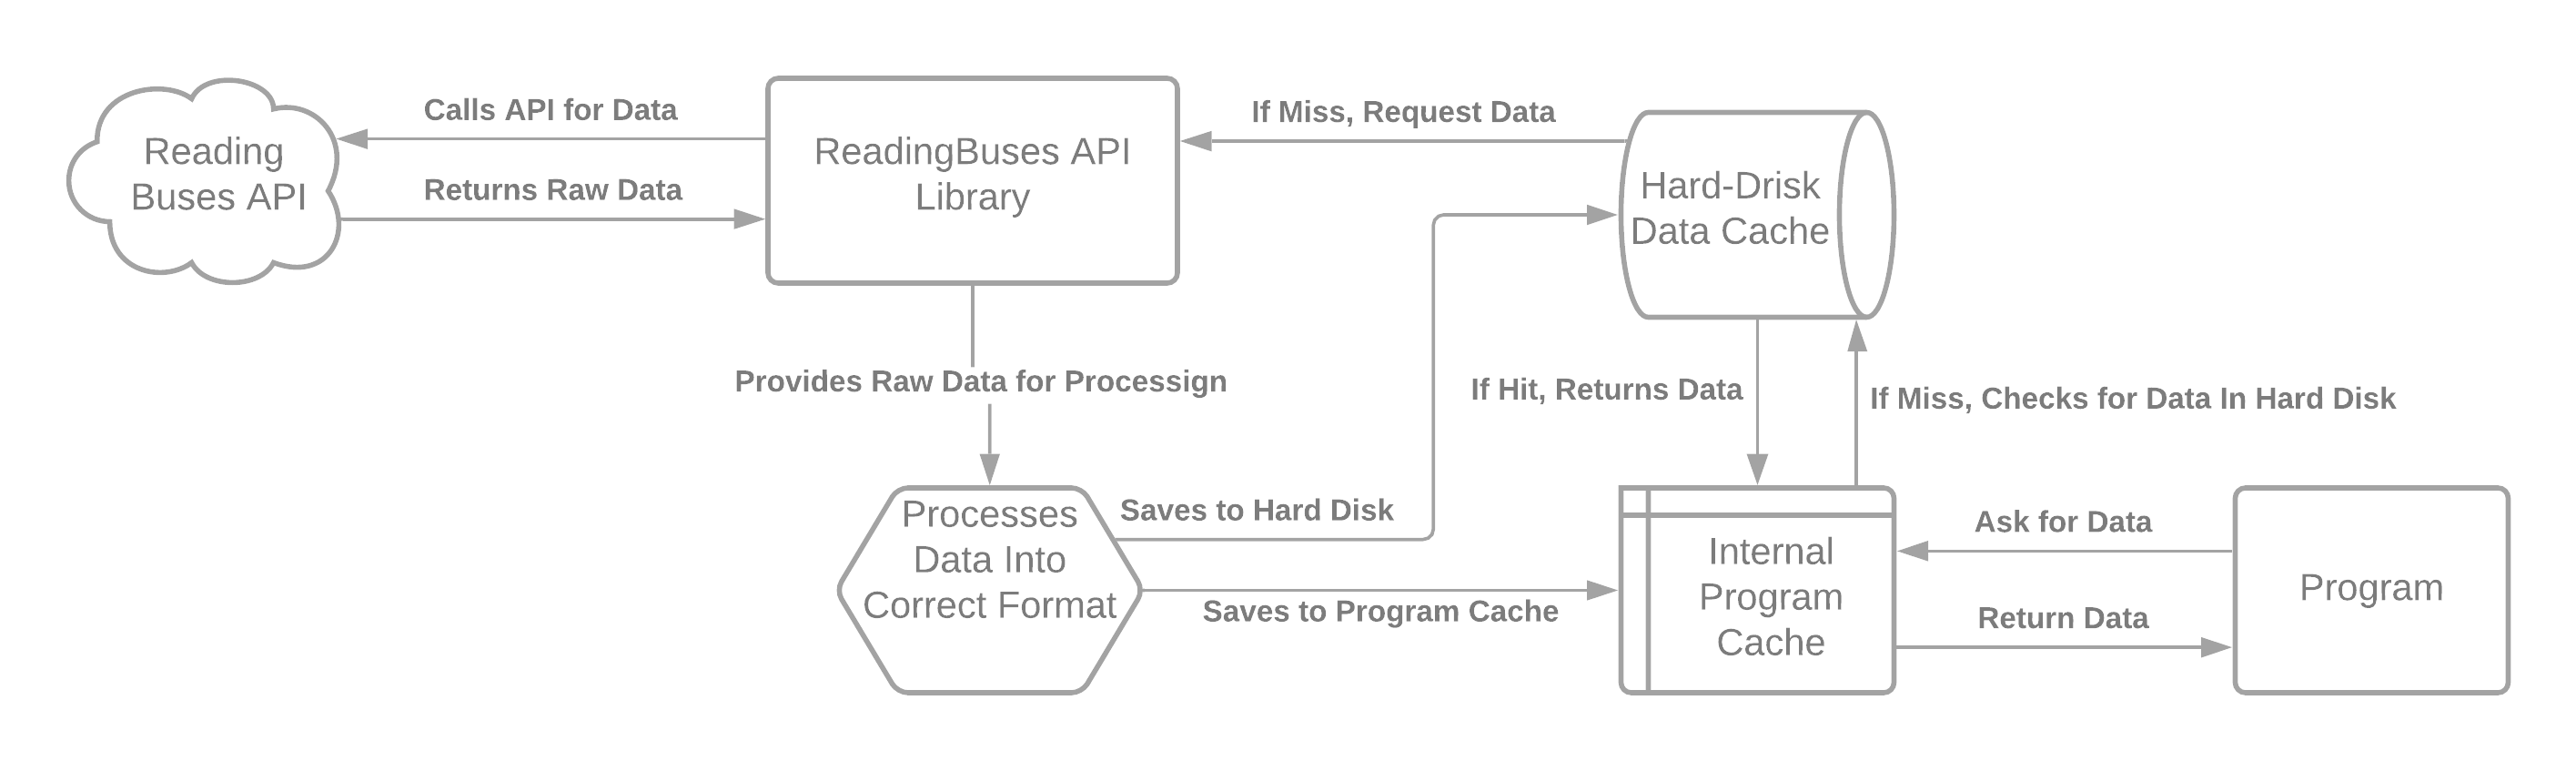
\includegraphics[width=400px]{images/cacheV2.png}
	\caption{Data Caching System Architecture}
	\label{fig:cachingsystem}
\end{figure}


I identified that making data request to the API was a bottleneck in the system, it would be completely impractical to request the volumes of data needed for the program every time it is run. Furthermore, historical data is not going to change after the date has taken place because the same result is always going to be returned I can simply cache it locally. 


\par 
I have developed the caching solution to be unobtrusive, abstracting out its complexity, so I can simply make method calls for data throughout the program, without having to worry about where the data is coming from or how. Data caching happens at two tiers, every time a data request is made, the program first checks to see if the data is held within its internal program cache. 

\par
This internal cache is managed using the ``\texttt{System.Runtime.Caching}'' library from Microsoft; the implementation for which can be found in my ``\texttt{InternalCache<T>}'' Class. First, it checks if the data is inside of the ``\texttt{MemoryCache}'' object, if not it then calls upon the function pointer provided to generate the data. This process is all secured with Concurrent Dictionaries and Semaphores to ensure thread-safe data access.


\par 
Data is retained within the program cache for 10 minutes since last being accessed, this should be long enough that it never expires between iterations of the search algorithm. While not posing too much of a risk exhausting system memory resources, with \CS \ restricting overall program memory usage to around 4GBs (per object).


\par 
 Internal program cache is required because I identified early into development using Visual Studios inbuilt debugging tools and the System.Diagnostics.StopWatch class that IO Operations and JSON parsing were taking a relatively long period of time, for the number of times they were being performed. Causing a system bottleneck that needed to be resolved.

\par 
If the data is not in the programs internal cache, it is checked in the secondary cache tier, which is saved directly onto a user hard drive. The files are saved as ``.cache'' hidden files, in a directory path local to the executing program, called ``cache'', separated by the Operator Name, and Service ID path. 

\par 
Most data should however be moved from the secondary cache into the internal program cache during the pre-evaluator checks stages, where it checks that all the required data is at least already in secondary cache.

\par 
If the data is also not in the secondary cache, then it is the first time the user has ever requested this data and as such a call must be made to the API feed. Once the data is returned back it is processed into the correct format for the program and then a copy is stored into both cache tiers for future use. Allowing for significantly faster data retrieval on all future subsequent requests of the data.

\par
Pre-Evaluator Checks are carried out at the start of performing every search to check what data is currently cached or not, caching all data before beginning the first iterations. This has two benefits, the speed of the search will be unimpeded once began and it allows for me to be able to calculate the performance metrics of the services current timetable with ease.  


\subsection{Asynchronous Data Management}
While I am caching the majority of the data, I cannot always assume a cache hit, and even if I have cached the file in secondary cache, reading from local storage and parsing the file into program memory can still take some time, especially for high-frequency services which will have a lot of data in a file to parse. As such, I needed to perform this work off of the main program thread, to prevent the GUI from freezing later on and to allow for me the ability to carry out several requests to the API simultaneously.  


\par 
I decided to achieve this with a Task-based Asynchronous Pattern (TAP)\cite{RN29}, through the use of \CS, \texttt{System.Threading.Tasks.Task\textless TResult\textgreater}  library. This allowed for me to be able to easily compartmentalise work into tasks, which can then be queued, run asynchronously and managed to wait for some, or all, to complete with ease. This is particularly useful when I want to get several dates' worth of data. Instead of doing each request sequentially and synchronously on the main thread, I can queue up all dates of tasks, and instruct them to all run concurrently on individual threads. With Tasks, abstracting much of the complexity away for me.  



\section{Evaluation}
The following section evaluates my aims and objectives of the project and any changes made from the original work plan. 

\subsection{Evaluation Of Aims And Objectives}
Overall I am very happy with the attainment of my original aims and objectives, I have completed almost all of my objectives and to a high standard. Below I shall evaluate each point from section \ref{aimsObjectivs}.

\par
For objective one, I successfully created a robust and efficient solution for interfacing with the API, including several systems such as data caching to speed up this process, as detailed in section \ref{caching}.

\par
For objective two, I identified points where timetables changed throughout the year and to great success, handling a range of outlier events such as Christmas and New Year well, as detailed in section \ref{timetablePatterens}.

\par
For objective three, I successfully generated previous performance metrics and these are displayed to the user before starting a new search. Moreover, the score of the initial input solution and the final solution is shown to the user, along with a colour highlighted timetable to show where the improvements have been made. 

\par 
For objective five, I calculated the objective score function value for the initial solution and final best solution, outputting the percentage change improvement to the end-user, allowing them to compare the estimated performances of both services. As such, I believe I have successfully achieved this goal.  



\subsubsection{Evaluation of Search Algorithm}
For objective four, I did successfully produce a search algorithm that was able to take in an initial solution and using a data-driven approach produce a new ``optimised timetable''.  I investigated several optimisation methods, considering local search methods, genetic algorithms and integer programming to meet the objective of the first sub-requirement ``A'', as explained in section \ref{strats}.

\par 
Sub-requirements ``B'' and ``C'' which relate to the first optimisation target, of altering slack and travel times for the services were achieved.  With each iteration of the search algorithm the objective score value for this target generally improved. As shown in the test data results in appendix section \ref{slackObj}.


\par 
While it is difficult to know with complete confidence how a bus would actually behave in the real world given the uncertainty of real-world conditions. I can still be very confident in my metrics to evaluate the solution as I minimise the total number of changes and use a large amount of historical data. As such I am very proud of my work in section \ref{simulation} and \ref{STOE} to address these requirements. 


\par 
To meet the Sub-requirement ``H'', which relates to the third optimisation target of ensuring a uniform distribution of services at a stop that share a common route-segment, significant work was performed on the identification of shared route segments. As explained in detail in section \ref{sharedRoute}, the identification of shared route-segments was very successful, with the majority of expected segments from intrinsic knowledge being found and identified by the program.



\par
The cohesion blame evaluator as detailed in section \ref{SCOE}, worked well for services that all diverge at the same location or where there was a small number of services sharing the same route-segment. The evaluator generally produced a plausible output, but would sometimes produce higher than expected values.

\par 
The main problems arose due to some services diverging off and creating unrealistic target times. As such, service cohesion was regrettably not used when making move decisions and so is no longer a part of the optimisation search.  

\par 
For sub-requirement ``I'', I allowed the algorithm to be parameterised, along with several other program settings, such that the end-user can tailor it to their needs and experiment based on how they want the search to function. For example, changing the weighting of the objective targets, the size of the neighbourhood, candidate list, tabu-tenure length and whether to use weak-stop data or not. A full list can be seen in Figure \ref{fig:settings}.

\par
All other sub-requirements were constraints I must place on the search and all of these were successfully met. 

\par
The tabu-list implementation was also very successful, with the search algorithm making a range of varied moves. Targeting all services included within the search, and for a range of different stops, directions and times of days; never getting stuck on one specific part of the solution. An example of moves made by the program can be shown in the appendix, section \ref{moveSummary}

\par 
Overall, I am very pleased with how the search algorithm resulted. I had an ambitious set of initial goals and achieved the majority of them. With the search algorithm successfully producing a new set of improved timetables. 


\subsubsection{User-interface and Experience Evaluation }
For objective six, I am very happy with the user interface I developed, while simplistic in parts, it is highly informative and intuitive in design. Significant time was invested to constantly inform the user on the progress of tasks, through the use of progress bars and text boxes. This was particularly important for very long-running tasks as it gives a level of comfort and assurance that the program is doing work in the background and gives an indication of how long you might have to wait. I am particularly proud of the search page, which informs in real-time if the solution is improving or not and of the timetable viewer screen, which lets the user clearly see the changes made and remaining trouble spots. A full set of program screenshots can be found in the Appendix Section \ref{screenshots}.




\subsection{Work-Plan Changes}
As the project progressed there were some minor changes from my original work plan to better reflect the changes in direction of the project. The first change was to expand out the ``slack'' time optimisation criteria to also include journey times. By including both the dwell and travel times, the new optimisation criteria can now be thought of as a measurement of how likely a service will be able to meet its scheduled timetable. Doing this adds an extra layer of complexity and makes for a more useful optimisation criteria to aim for.

\par 
I removed from the project scope, the fourth optimisation target of aiming for specific target times. However, this was no longer needed as my understanding of service cohesion evolved and I learnt this could lead to a lot of conflictions with the first objective target.


\subsection{Testing Strategy}
\label{testing}
My Testing strategy is split between the two projects in the Visual Studio Solution, the first project contains the Reading Buses API Library and the second the actual Time Table Optimiser Program.   


To test the Reading Buses library I have written Unit-Tests for each class, including any communication between them. Each test has a ``live'' and ``dummy'' pair associated. The live tests, call upon the real API feed, making and receiving an actual request for data. This allows me to ensure the library is working as intended. Although, response times can be very long, taking up to 15 minutes for all tests to complete. As such I also have associated dummy tests, these do not call upon the live server, instead, they call upon my hosted data-store of static results.

\par 
This has two main benefits, first the response times are significantly quicker, with the only bottleneck being the internet connection, as opposed to the server response time. Therefore, I could test and check the library is working much faster than beforehand, speeding up development. Secondly, if my dummy tests pass, but my live tests fail it allowed for me to easily identify if the live server might have updated its data-schema, as opposed to an error being in my code. 

\par
A Continuous Integration Pipeline was set up onto the master branch in GitHub, allowing me to quickly identify and fix any issues I may have accidentally introduced. 

\par
To test the main program I had originally envisioned a combination of unit, integration and performance tests. Unfortunately, it soon became apparent that generating fake data was a long and laborious process, often taking longer to produce the data than to write the test. This was particularly true for parts of the system that relied upon the output of others, such as the cohesion service evaluator that needed to take in route design and timetables for those routes. 

\par 
As a proof of concept I have written a few unit tests to demonstrate how these could be achieved, but due to time constraints and because this is not meant to be a commercial system, I was unable to have full formal unit and integration test coverage. The majority of bugs I encountered were null-reference related, which is why I enabled nullable types early into the project, see section \ref{null} for more information.

\par 
Throughout development, I made use of Visual Studios industry-leading debugging tools, such as breakpoints, data inspection, object watching and events viewer. To help understand the state of the program during runtime. However, this was sometimes challenging as there were so many timetable record and weight objects that it was difficult to understand the larger picture of how they were changing.

\par 
As such, I employed the less formal use of exporting data to CSV format to inspect in Microsoft Excel, this was particularly useful in helping to identify trends in the large volumes of data. By allowing me to quickly plot out several graphs and using conditional formatting to colour highlight cells. Eventually, I designed my own in-built system, in the timetable viewer that would colour cells, from green to red, depending on their squeaky wheel blame value for the different objective functions. 


\begin{figure}[H]
	\centering
	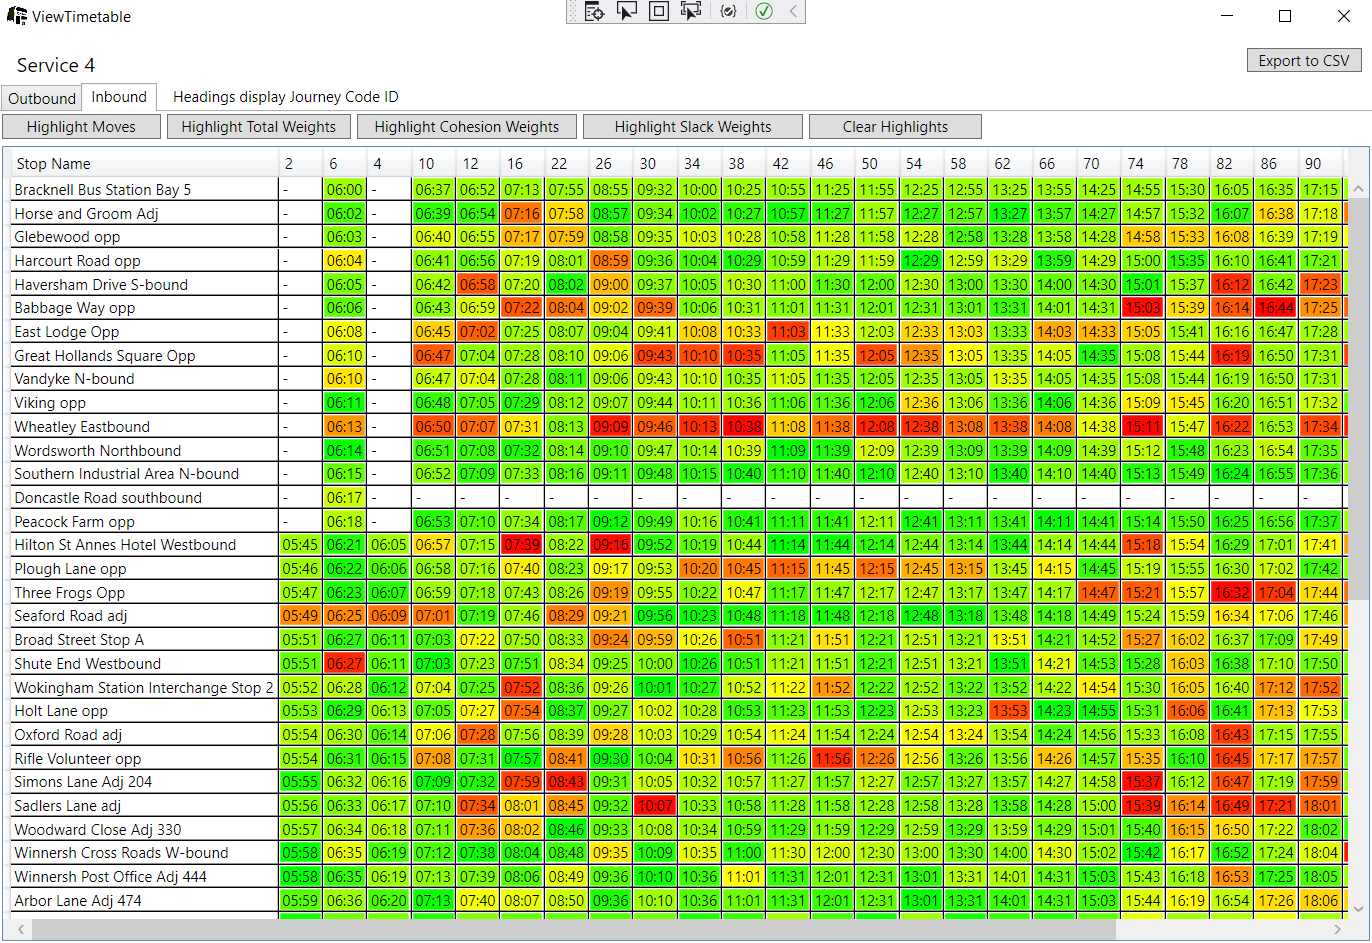
\includegraphics[width=300px]{images/cellhighlights.png}
	\caption{Timetable Viewer Conditional Highlighting Window}
	\label{fig:highlighting}
\end{figure}


\par 
This significantly speeded up my process, removing the need for Excel conditional formatting and allowed me to see at each iteration visually the changes to the weightings of different records automatically. Something which would not have been possible using Visual Studios inbuilt debugging tools, due to the volume and complexity of data being changed. 

\par
While I predominately worked on data for the month of May and for services in East of Reading, due to my familiarity with the services, I also tested the program using data from various other points of the year and for services across all parts of Reading; to ensure that it worked as expected for other data-sets.


\par 
Performance testing was carried out throughout development, which can be categorised into two stages, API Performance Bottleneck \& Capability Testing and Program Evaluation Performance Testing. 

\par 
The API performance and bottleneck testing involved establishing the rate limits and best combination of concurrent request, something which was not clearly documented. It became apparent that there was no daily rate limit, or concurrent request limit. But making several concurrent requests was not always faster than queueing them sequentially. The perfect degree of parallelism was around 3-5 concurrent requests. An interesting quirk of the API was sending the exact same request twice (or more) concurrently would cause both to fail. It was therefore important to ensure between threads that the same request was not already being awaited. 

\par 
Program Evaluation Performance Testing was informally performed to ensure the program could handle both the scale and volume of data required. It became quickly evident that the API was the largest bottleneck in the system, which is why a multi-tiered caching solution has been implemented; please refer to section \ref{caching}. Along with concepts such as ``Weak Stop'' data, to limit having to ever query the API in the first place and carefully tracking the changes between iterations, only re-evaluating what is truly necessary; limiting unneeded computation.

\par 
Progress bars and reports could also be used to see what parts of the program were taking the longest, to target for improvement where possible. 

\paragraph{Performance Metric Results}

Overall, I am very happy with the performance of the program, improvements to an initial solution can be found in a reasonable amount of time given the large quantities of data being processed to generate a result. The performance results can be found in the Appendix Section \ref{performance}. This shows that iteration time increases as you increase the number of services, days or data and candidate list size, as expected.


\subsubsection{Nullability}
\label{null}
For this project I enabled \CS 8, ``Nullability'' feature \cite{RN41}, which required me to specifically annotate every variable with a ``\texttt{?}'' if it can be null or not. This helped significantly with my overall code quality, as it forced me to provide an alternative non-null value whenever trying to convert between nullable data types. Ensuring that I never missed a segment of code that might result in a null-pointer exception. Moreover, it helped me to identify and consider what should happen in several outlier events; particularly important where the API provides unexpected data. 





\section{Summary and Reflections}

I shall now summarise and reflect upon my work in this project.


\subsection{Data Quality Issues} 
One area which hindered my progress was the quality of the data, throughout development, I uncovered several data issues, such as erroneous arrival and departure times, erroneous data about the last and first stops on all services journeys, missing data, data about wrong services being returned by the API, data about the wrong stops being returned by the API and incorrect route layouts within the API. The consequence of poor data quality was it required several hours of testing and investigation to discover issues that were not within my code, but instead within the data. This wasted time could have been better spent on development elsewhere in the program.  


\subsubsection{Data Mitigation Strategy}
To mitigate data quality issues I deployed several different strategies throughout the program. To deal with erroneous data I would normally remove the top and bottom five percentile of results and prevented the search from selecting the first or last stop as a target record for a move, this normally proved sufficient. To deal with any missing data I would try and fill it in with an average value or remove it from the data set where possible. To deal with information about the wrong service or stop being returned by the API, I made checks throughout the program to ensure the result is what I expected it to be. 


\subsection{Data Volume Issues}
Another area that slowed down the progress was the volumes of data, as explained in section \ref{testing}, testing was very difficult and a lot of time was required to develop the caching solution I now have in place. Another issue it caused was with executing the program, while one iteration of a small search would take only one to two minutes this would start to add up and slowed down my ability to be able to quickly run and test the program between changes. 

\subsection{Contingency Data-Backup}

At the start of the project, I backed up a year's worth of historical timetable data for several popular routes throughout Reading, privately onto both cloud and local storage systems. In the event that the Reading Buses Open Data API becomes unavailable for whatever reason, this data could then simply be placed into the programs cache folder and I could continue relatively unaffected. This decision proved fruitful as Reading Buses decided upon shutting down their API on the 4th of April 2021, thankfully, I was not affected by this decision due to my forward-thinking.


\subsection{Reflection on Methodology and Design}
Overall I am content with my methodology and design selected, Tabu-Search is a relatively unused search algorithm in timetable optimisation and as such, I provided a new and viable novel solution to the problem.  Wei Fan \textsl{et al} has proposed Tabu-Search for transport network optimisation with variable transit demand \cite{RN25}, but this focused more upon the design of the network. To my knowledge, there is no published data-driven tabu-search bus timetable optimisation work.

\par
Several design patterns are used throughout the codebase, such as the Singleton, Factory, MVVM and Facade with great effect. Moreover, all code has been commented and therefore, I believe that I have produced high-quality, maintainable and extendable code for any future development. 


\par 
For future research, I could explore intensification to return back to previously promising areas and explore them further. I could also investigate an aspiration criteria to override the tabu-list if a move is sufficiently good. Furthermore, I could improve the total blame calculation and examine more complex methods for service cohesion evaluation. 


\subsection{Reflection on Chosen Technologies}

Overall I am happy with my chosen technologies, \CS \ and particularly \texttt{LINQ} allowed me to be able to quickly produce solutions to problems with ease, due to its initiative syntax and declarative abilities. However, one area of \CS \ that was challenging was with ``cloning'', at different points in the program shallow and deep cloning was required of parts or entire solution objects. Conceptually keeping track of what objects were clones or where the same was very difficult. If I had the time C++, would have made memory management more efficient, but it would have also taken much longer to produce a solution in; when taking this into account, I made the right choice. 


\subsection{Project Management}
Throughout the project I have had bi-weekly meetings with my project supervisor, where I outlined the work I had completed in the previous two weeks and the scope of the work intended to carry out during the following two weeks, using my work-plan, shown in Figure \ref{fig:workPlan} to guide me. I split the problem up into discrete parts and outlined to myself when I wished to have it completed by, in a SCRUM like agile approach.

\begin{figure}[H]
	\centering
	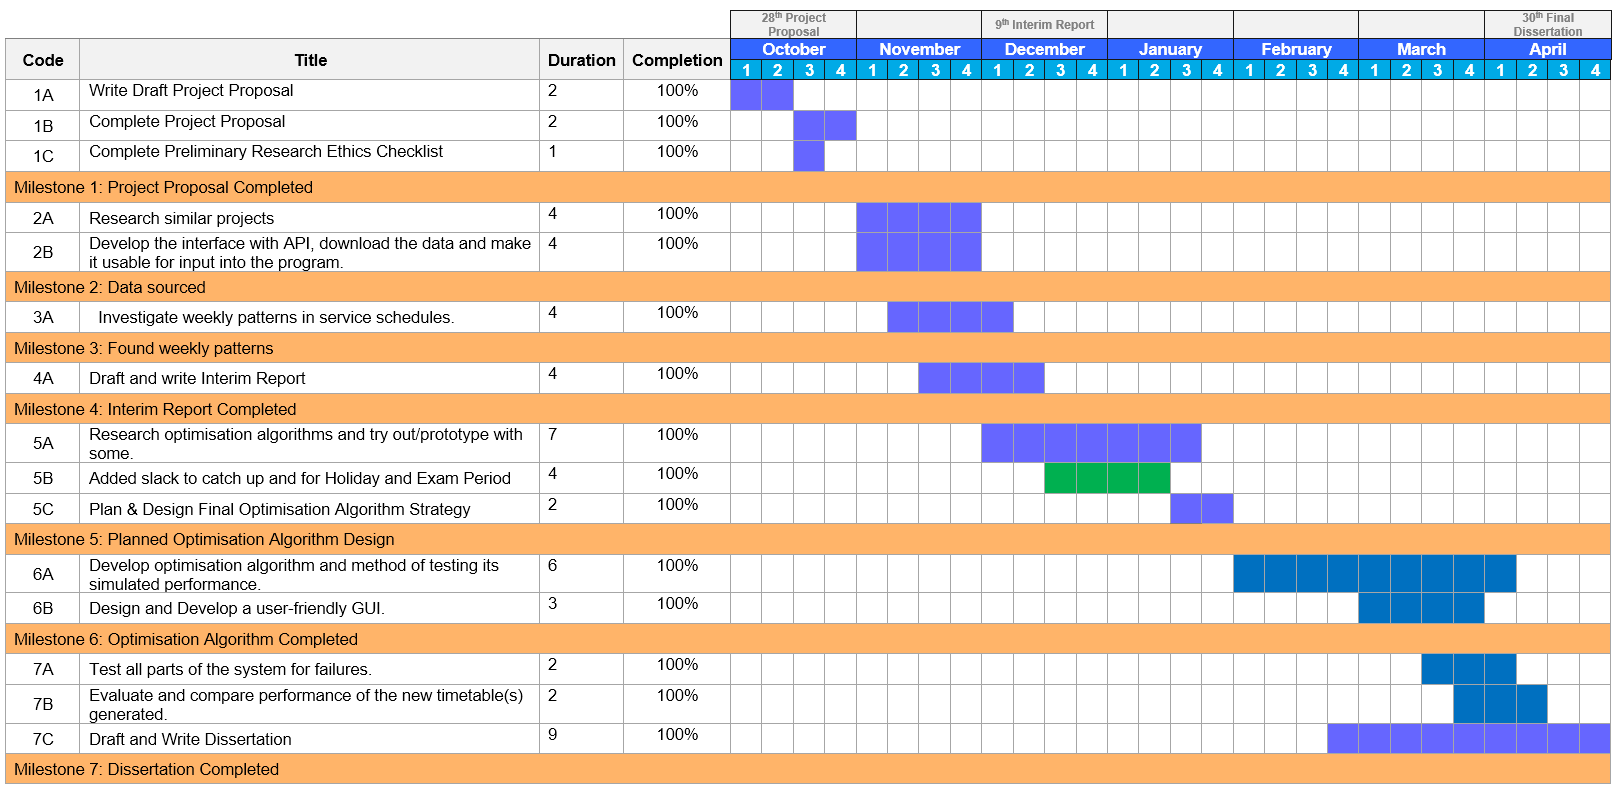
\includegraphics[width=400px]{images/ganntChartV4.PNG}
	\caption{Gannt Chart Work Plan For Project.}
	\label{fig:workPlan}
\end{figure}


\par 
For the project, I used Azure DevOps to manage my work items in a more efficient and structured way, particularly when I was less experienced in approach and the complexity of the task grew. Azure DevOps enabled the use of an easy to read and edit digital kanban like board to manage workflow, priorities, estimated time and dependencies/relations on other items. My kanban board had four columns, ``To-do'', ``in-progress'', ``testing'' and ``completed'', for which I would move my work items between during each sprint. 


\par 
My Azure DevOps Project integrated well with Microsoft Excel and Project, which I used to input in my project timelines and work items. I chose to use Azure DevOps as it is a popular choice in industry, I had previous development experience using it and it works well with my other technologies chosen (Visual Studio and Git.)

\par
Research papers and references were stored using EndNote, which ensured a consistent reference convention and let me add a rating, highlight and make notes on the papers I read.  

\par 
The code was hosted on both my own personal GitHub account and mirrored on the schools' Git Labs server, for an extra layer of backup protection. Around 300 frequent and regular commits were made, with branches used when developing a new feature or experimenting with possible alternative solutions. Git enabled me to easily manage my code base and provided me with the ability to return to previous commits if something broke.


\par 
There were points where I missed my original work deadlines, primarily due to unanticipated difficulties, greater than expected work commitments for my other modules and the challenges associated with a completely online year. However, this work was soon caught up on and I am very happy with the level of work completed and my overall progress.


\par
A key lesson I learnt was the importance of having a clear starting vision and the need for contingency in the work plan. If I was to start the project again, I would narrow down my vision sooner and give myself more contingency periods to enable me to catch up on any work that might overrun.


\subsection{Future Usage and Scope}
I think that my project has many possible new exciting areas of future use and research. It was designed from the start to be able to work with any other bus operators API and should another operator wish to use this program switching to it from the Reading Buses API would be a very quick and simple procedure, with the Bus Operator Factory object needing only minor changes. 


\par 
Moreover, while the project was envisaged for use with buses, there are many similarities between a bus timetable and other public transports modes such as trams and trains. Trams and Trains both share route-segments, perhaps more so than buses, with shared routes being even more common, for example, there are several services from Reading to London per hour. Both trams and trains also require dwell time and could have their journey times evaluated with historical data. As such, you could consider bus stops and stations to be conceptually quite similar, providing a possible new area of research for future work.


\subsection{Contributions and Reflections}
Upon reflection, I am very happy with the outcome of my project, I set myself an ambitious set of tasks and completed almost all of them and to a very high standard. 

\par
Data-driven approaches to bus-timetable optimisation is still a very under-researched area, particularly so for UK bus networks. However, with the introduction of the Bus Services Act, 2017 \cite{RN13} requiring UK operators to start publishing open data and with 98\% of UK buses now equipped with AVL technology as of 2020\cite{RN12}, I envision this to be an exciting expanding area of future research. 

\par 
Throughout the project, I have developed my skills and knowledge, including the ability to effectively conduct independent research and knowledge of different search algorithms. I now have a much greater understanding of the complexity of timetables, how one single change causes changes throughout the solution and that there are internal and external factors to consider when developing a new timetable.


\par
I now also have a greater appreciation for the complexity of handling such large volumes of data, understanding the importance of creating an efficient solution to process the data, keep track of changes, being able to filter and remove erroneous data, identify edge cases, spot trends in the data and test a solution to ensure it works correctly.


\par 
I consider I have achieved two main contributions, the first being my research in the use of tabu-search in a data-driven approach to bus timetable optimisation. As aforementioned, data-driven approaches are still relatively new, but the methods that do exist most commonly utilise genetic algorithms. Tabu-search is a very under-utilised search algorithm and I have demonstrated its viability and opened up future possibilities to explore more advance uses such as the addition of intensification and an aspiration criteria. 

\par
My second main contribution is the exploration of different services that share a common-route segment. While there is a lot of research performed on transport route-network design, there is limited research on the cohesion of services that share a common segment of stops. Something, which I believe is becoming increasingly common, particularly in urban locations where bus lanes are more prevalent. 

\par 
I have proposed a solution to identifying and analysing the cohesion of services in a shared route segment. While also discovering and discussing several troublesome areas that would need to be tackled in future research. As such, I have targeted several under-researched areas and provided a unique and interesting solution to a novel and challenging problem. 

\par
Moreover, I believe that my program has many exciting future usages either with other bus operators API feeds or with research into using it with other public transportation modes, such as trams and trains. 

\par 
In conclusion, bus timetable optimisation is a very complex problem, but I have been successful in my ambitions for the project and this has been a very rewarding experience. Creating a solution that is capable of optimising a timetable based upon the three optimisation criteria specified. A bus operator could use my final program to help aid their decision making when producing a new timetable, therefore, I believe I have successfully met my overarching goal of the project. Moreover, I have targeted several under-researched areas and contributed a new and novel approach to the problem. 



\newpage

% Do this to get it to show up in the contents page.
\phantomsection
\addcontentsline{toc}{section}{References}
\printbibliography %[heading=none]


\newpage
\pagenumbering{roman}


\section*{Appendices}
\addcontentsline{toc}{section}{Appendices}
\setcounter{section}{8}
\setcounter{subsection}{0}
%
%\begin{itemize}
%	\item Was considering moving Pseduo-code blocks here
%	\item Was considering adding screenshots of the GUI here.
%	\item Was considering adding some example/sample raw data from the API here.
%	\item Explain the software settings page here.
%	\item If I had time, a very very brief user manual...
%\end{itemize}


\subsection{Program Screenshots}
\label{screenshots}
\begin{figure}[H]
	\centering
	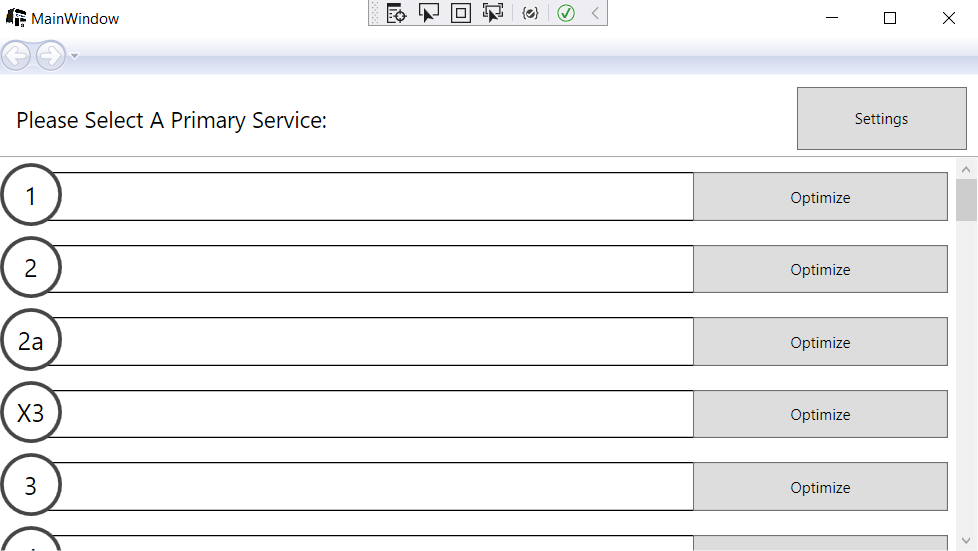
\includegraphics[width=400px]{images/mainPage.PNG}
	\caption{The Main Start Screen of The Program}
	\label{fig:mainPage}
\end{figure}

\begin{figure}[H]
	\centering
	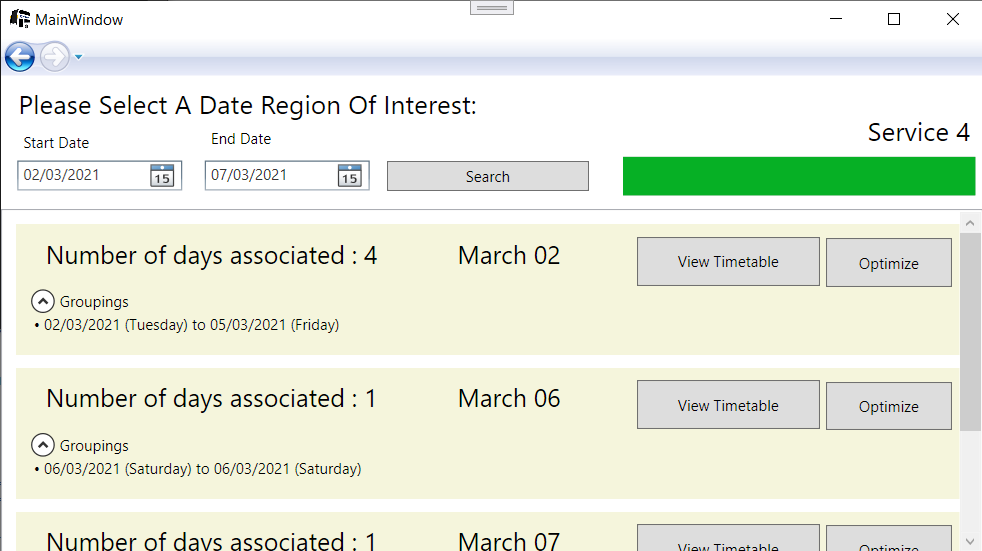
\includegraphics[width=400px]{images/dateTimeSelector.PNG}
	\caption{Date Region Selector Screen}
	\label{fig:dateSelector}
\end{figure}

\begin{figure}[H]
	\centering
	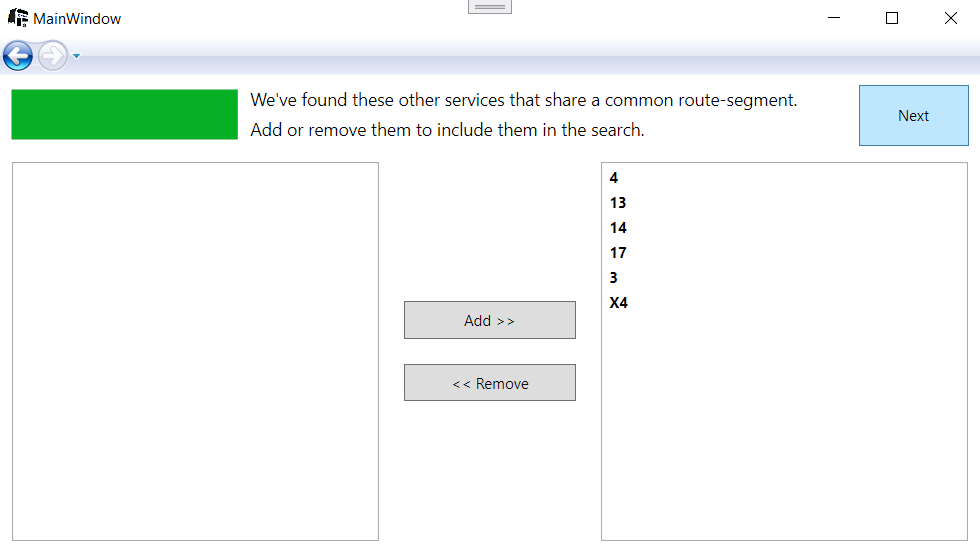
\includegraphics[width=400px]{images/routesegment.PNG}
	\caption{Route Segment/ Service Selector}
	\label{fig:routeSegmentSelector}
\end{figure}

\begin{figure}[H]
	\centering
	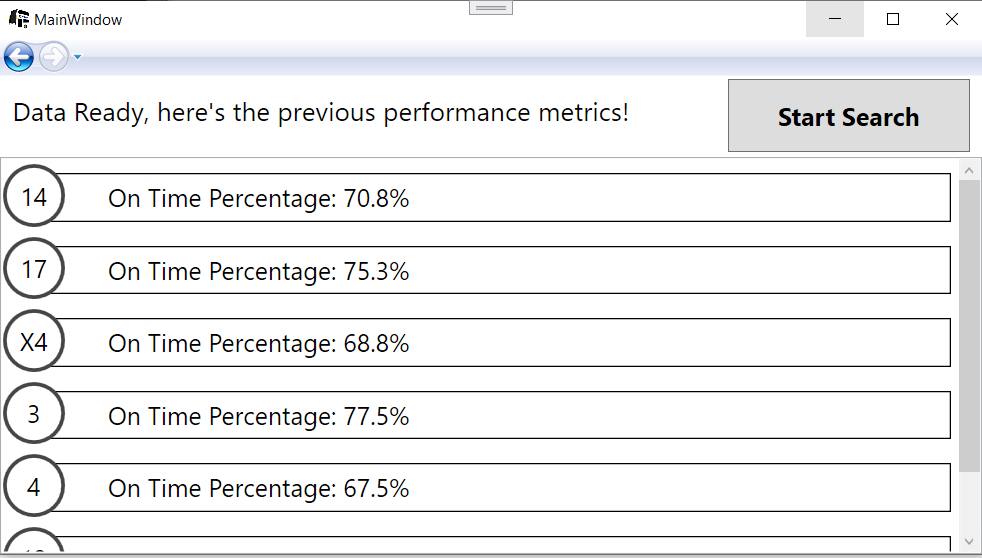
\includegraphics[width=400px]{images/performance.PNG}
	\caption{Previous Performance Metrics Page}
	\label{fig:performanceMetrics}
\end{figure}

\begin{figure}[H]
	\centering
	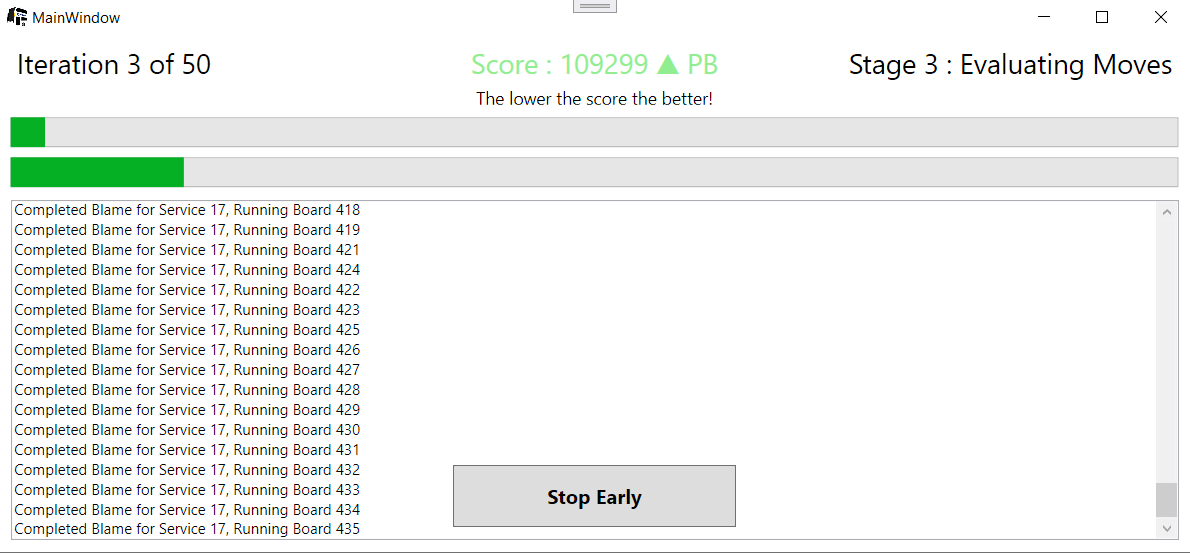
\includegraphics[width=400px]{images/searchScreen.PNG}
	\caption{Search Screen}
	\label{fig:searchScreen}
\end{figure}

\begin{figure}[H]
	\centering
	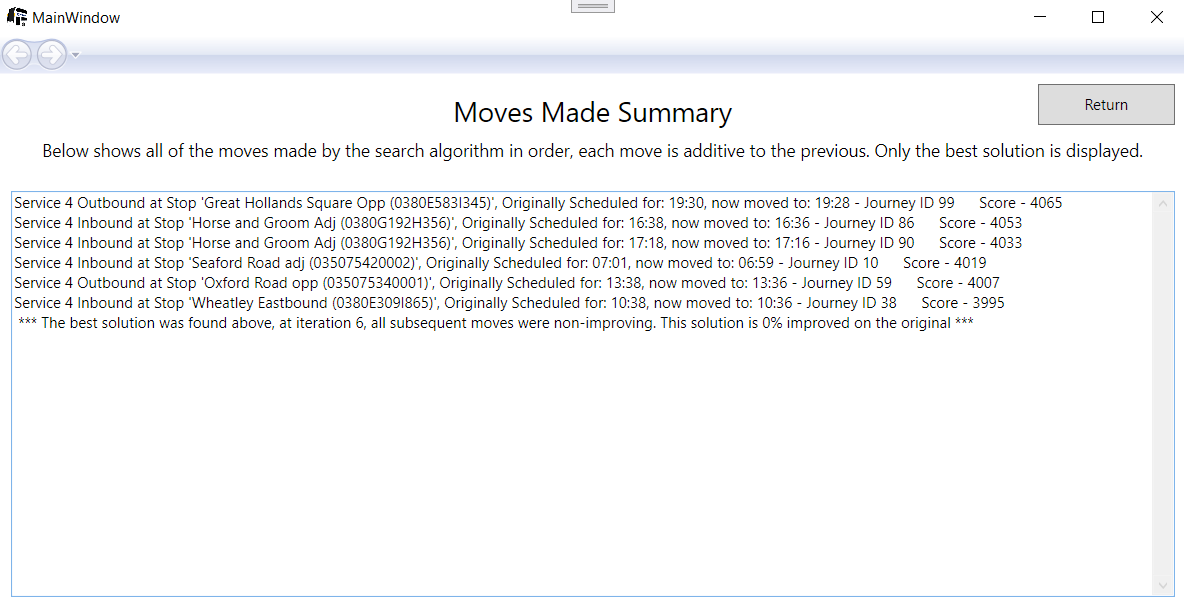
\includegraphics[width=400px]{images/movesmade.PNG}
	\caption{Moves Made Page}
	\label{fig:movesMade}
\end{figure}

\begin{figure}[H]
	\centering
	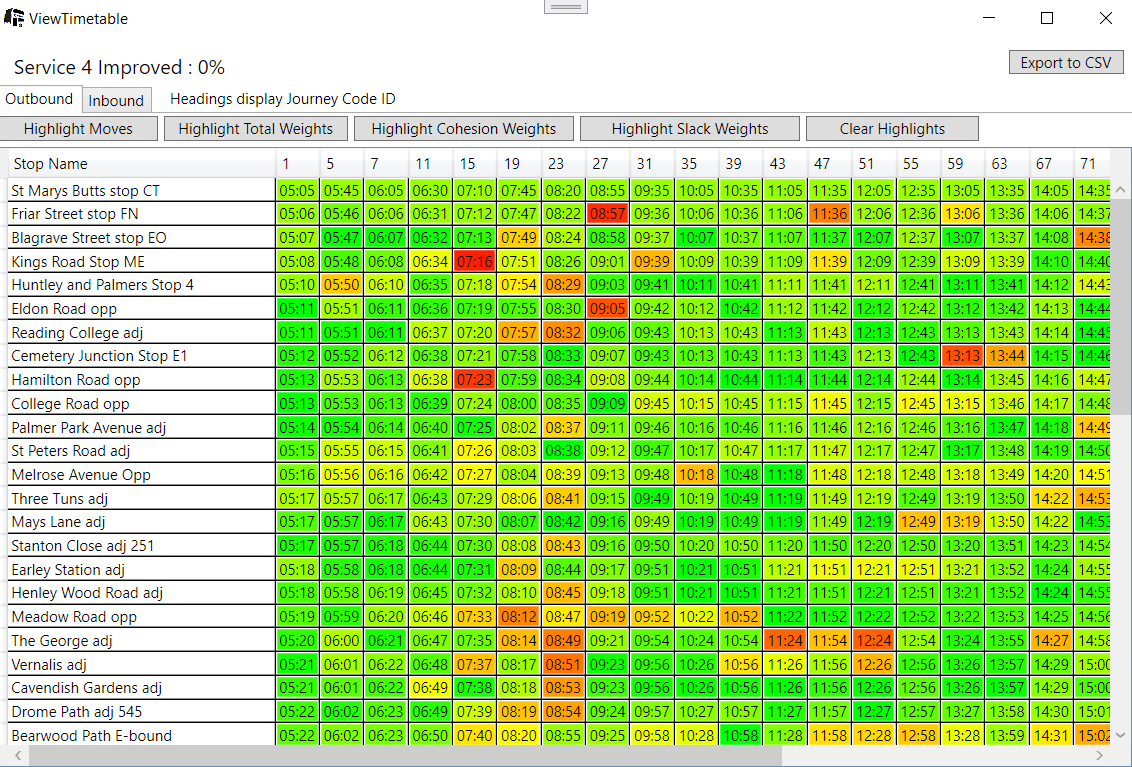
\includegraphics[width=400px]{images/timetableviewer.PNG}
	\caption{Timetable Viewer}
	\label{fig:timetbaleViewer}
\end{figure}


\begin{figure}[H]
	\centering
	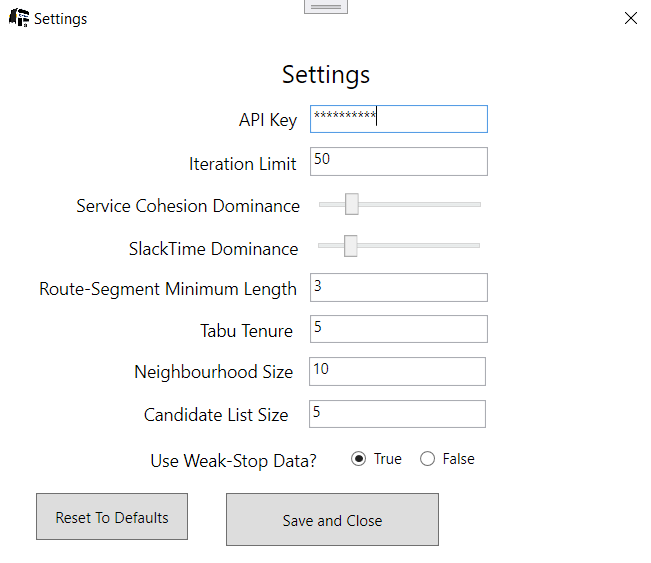
\includegraphics[width=250px]{images/SettingsPage.PNG}
	\caption{Settings Page}
	\label{fig:settings}
\end{figure}

\newpage

\subsection{Performance Results}
\label{performance}

All tests were ran on the same device, running an Intel i7 4770k with 16GB RAM on Windows 10 Pro 64bit. While running times are not the same for all tests, the speed for the number of iterations should be fairly consistent and so a reasonable average can still be made.  

\begin{figure}[H]
	\centering
\begin{tabular}{|l|l|l|l|l|l|}
	\hline
	\multicolumn{1}{|c|}{\textit{Services}} & \multicolumn{1}{c|}{\textit{\begin{tabular}[c]{@{}c@{}}Date\\ Range\end{tabular}}} & \multicolumn{1}{c|}{\textit{\begin{tabular}[c]{@{}c@{}}Candidate\\ List size\end{tabular}}} & \multicolumn{1}{c|}{\textit{\begin{tabular}[c]{@{}c@{}}Running\\ Time\end{tabular}}} & \multicolumn{1}{c|}{\textit{\begin{tabular}[c]{@{}c@{}}Iteration \\ Count\end{tabular}}} & \multicolumn{1}{c|}{\textit{\textbf{\begin{tabular}[c]{@{}c@{}}Iterations \\ per hour\end{tabular}}}} \\ \hline
	3, 4, X4, 13, 14, 17                    & 1 Month                                                                            & 5                                                                                           & 7 hours                                                                              & 21                                                                                       & 3                                                                                                     \\ \hline
	3, 4, X4, 13, 14, 17                    & 1 Week                                                                             & 5                                                                                           & 4 hours                                                                              & 43                                                                                       & 10.8                                                                                                  \\ \hline
	3, 4, X4, 13, 14, 17                    & 1 Day                                                                              & 5                                                                                           & 1 hour                                                                               & 51                                                                                       & 51                                                                                                    \\ \hline
	4, X4                                   & 1 Week                                                                             & 5                                                                                           & 2 hours                                                                              & 104                                                                                      & 52                                                                                                    \\ \hline
	3, 4, X4, 13, 14, 17                    & 1 Week                                                                             & 2                                                                                           & 1 Hour                                                                               & 68                                                                                       & 68                                                                                                    \\ \hline
\end{tabular}
	\caption{Performance Test Results}
\end{figure}




\subsection{Slack and Travel Time Test Results}
\label{slackObj}

The first test was performed on services 3, 4, X4, 13, 14, 17, on one month of data and a candidate list of five. It shows every move made is a positive, improving move, with the objective function score decreasing. 

\begin{figure}[H]
	\centering
\begin{tabular}{|l|l|l|} 
	\hline
	\begin{tabular}[c]{@{}l@{}}Iteration~\\Count\end{tabular} & \begin{tabular}[c]{@{}l@{}}Objective Function\\Score\end{tabular} & Change  \\ 
	\hline
	1                                                         & 56153                                                             & 0       \\ 
	\hline
	2                                                         & 56139                                                             & 14      \\ 
	\hline
	3                                                         & 56128                                                             & 11      \\ 
	\hline
	4                                                         & 56114                                                             & 14      \\ 
	\hline
	5                                                         & 56106                                                             & 8       \\ 
	\hline
	6                                                         & 56094                                                             & 12      \\ 
	\hline
	7                                                         & 56079                                                             & 15      \\ 
	\hline
	8                                                         & 56072                                                             & 7       \\ 
	\hline
	9                                                         & 56061                                                             & 11      \\ 
	\hline
	10                                                        & 56051                                                             & 10      \\ 
	\hline
	11                                                        & 56045                                                             & 6       \\ 
	\hline
	12                                                        & 56034                                                             & 11      \\ 
	\hline
	13                                                        & 56028                                                             & 6       \\ 
	\hline
	14                                                        & 56023                                                             & 5       \\ 
	\hline
	15                                                        & 56018                                                             & 5       \\ 
	\hline
	16                                                        & 56008                                                             & 10      \\ 
	\hline
	17                                                        & 56001                                                             & 7       \\ 
	\hline
	18                                                        & 55995                                                             & 6       \\ 
	\hline
	19                                                        & 55983                                                             & 12      \\ 
	\hline
	20                                                        & 55977                                                             & 6       \\ 
	\hline
	21                                                        & 55968                                                             & 9       \\
	\hline
\end{tabular}
	\caption{Objective Function One, Test One}
\end{figure}




\newpage

The second test was performed on services 3, 4, X4, 13, 14, 17, on one week of data and a candidate list of five. Again, it shows every move made is a positive, improving move, with the objective function score decreasing. 

\begin{figure}[H]
	\centering
	\begin{tabular}{|l|l|l|} 
		\hline
		Iteration Count & Objective Function Score & Change  \\ 
		\hline
		1               & 54385                    & 0       \\ 
		\hline
		2               & 54377                    & 8       \\ 
		\hline
		3               & 54370                    & 7       \\ 
		\hline
		4               & 54361                    & 9       \\ 
		\hline
		5               & 54352                    & 9       \\ 
		\hline
		6               & 54344                    & 8       \\ 
		\hline
		7               & 54334                    & 10      \\ 
		\hline
		8               & 54326                    & 8       \\ 
		\hline
		9               & 54304                    & 22      \\ 
		\hline
		10              & 54298                    & 6       \\ 
		\hline
		11              & 54292                    & 6       \\ 
		\hline
		12              & 54280                    & 12      \\ 
		\hline
		13              & 54268                    & 12      \\ 
		\hline
		14              & 54253                    & 15      \\ 
		\hline
		15              & 54233                    & 20      \\ 
		\hline
		16              & 54217                    & 16      \\ 
		\hline
		17              & 54203                    & 14      \\ 
		\hline
		18              & 54192                    & 11      \\ 
		\hline
		19              & 54184                    & 8       \\ 
		\hline
		20              & 54175                    & 9       \\ 
		\hline
		21              & 54165                    & 10      \\ 
		\hline
		22              & 54150                    & 15      \\ 
		\hline
		23              & 54140                    & 10      \\ 
		\hline
		24              & 54088                    & 52      \\ 
		\hline
		25              & 54072                    & 16      \\ 
		\hline
		26              & 54052                    & 20      \\ 
		\hline
		27              & 54045                    & 7       \\ 
		\hline
		28              & 54039                    & 6       \\ 
		\hline
		29              & 54028                    & 11      \\ 
		\hline
		30              & 54013                    & 15      \\ 
		\hline
		31              & 53996                    & 17      \\ 
		\hline
		32              & 53981                    & 15      \\ 
		\hline
		33              & 53965                    & 16      \\ 
		\hline
		34              & 53948                    & 17      \\ 
		\hline
		35              & 53931                    & 17      \\ 
		\hline
		36              & 53914                    & 17      \\ 
		\hline
		37              & 53907                    & 7       \\ 
		\hline
		38              & 53892                    & 15      \\ 
		\hline
		39              & 53885                    & 7       \\ 
		\hline
		40              & 53874                    & 11      \\ 
		\hline
		41              & 53868                    & 6       \\ 
		\hline
		42              & 53859                    & 9       \\ 
		\hline
		43              & 53851                    & 8       \\
		\hline
	\end{tabular}
	\caption{Objective Function One, Test Two}
\end{figure}
\newpage


The third test was performed on only services 4, X4 on one week of data and a candidate list of five. Once again, it shows every move made is a positive, improving move, with the objective function score decreasing. 


\begin{center}
	\begin{longtable}{|l|l|l|} 
		\hline
		\begin{tabular}[c]{@{}l@{}}Iteration \\Count\end{tabular} & \begin{tabular}[c]{@{}l@{}}Objective Function\\~Score\end{tabular} & Change  \\ 
		\hline
		1                                                         & 6252                                                               & 0       \\ 
		\hline
		2                                                         & 6227                                                               & 25      \\ 
		\hline
		3                                                         & 6214                                                               & 13      \\ 
		\hline
		4                                                         & 6198                                                               & 16      \\ 
		\hline
		5                                                         & 6193                                                               & 5       \\ 
		\hline
		6                                                         & 6186                                                               & 7       \\ 
		\hline
		7                                                         & 6166                                                               & 20      \\ 
		\hline
		8                                                         & 6153                                                               & 13      \\ 
		\hline
		9                                                         & 6140                                                               & 13      \\ 
		\hline
		10                                                        & 6127                                                               & 13      \\ 
		\hline
		11                                                        & 6119                                                               & 8       \\ 
		\hline
		12                                                        & 6110                                                               & 9       \\ 
		\hline
		13                                                        & 6105                                                               & 5       \\ 
		\hline
		14                                                        & 6087                                                               & 18      \\ 
		\hline
		15                                                        & 6082                                                               & 5       \\ 
		\hline
		16                                                        & 6063                                                               & 19      \\ 
		\hline
		17                                                        & 6051                                                               & 12      \\ 
		\hline
		18                                                        & 6037                                                               & 14      \\ 
		\hline
		19                                                        & 6019                                                               & 18      \\ 
		\hline
		20                                                        & 6010                                                               & 9       \\ 
		\hline
		21                                                        & 6003                                                               & 7       \\ 
		\hline
		22                                                        & 5985                                                               & 18      \\ 
		\hline
		23                                                        & 5975                                                               & 10      \\ 
		\hline
		24                                                        & 5959                                                               & 16      \\ 
		\hline
		25                                                        & 5949                                                               & 10      \\ 
		\hline
		26                                                        & 5926                                                               & 23      \\ 
		\hline
		27                                                        & 5905                                                               & 21      \\ 
		\hline
		28                                                        & 5886                                                               & 19      \\ 
		\hline
		29                                                        & 5870                                                               & 16      \\ 
		\hline
		30                                                        & 5862                                                               & 8       \\ 
		\hline
		31                                                        & 5856                                                               & 6       \\ 
		\hline
		32                                                        & 5827                                                               & 29      \\ 
		\hline
		33                                                        & 5815                                                               & 12      \\ 
		\hline
		34                                                        & 5808                                                               & 7       \\ 
		\hline
		35                                                        & 5791                                                               & 17      \\ 
		\hline
		36                                                        & 5773                                                               & 18      \\ 
		\hline
		37                                                        & 5762                                                               & 11      \\ 
		\hline
		38                                                        & 5752                                                               & 10      \\ 
		\hline
		39                                                        & 5743                                                               & 9       \\ 
		\hline
		40                                                        & 5733                                                               & 10      \\ 
		\hline
		41                                                        & 5722                                                               & 11      \\ 
		\hline
		42                                                        & 5716                                                               & 6       \\ 
		\hline
		43                                                        & 5709                                                               & 7       \\ 
		\hline
		44                                                        & 5690                                                               & 19      \\ 
		\hline
		45                                                        & 5682                                                               & 8       \\ 
		\hline
		46                                                        & 5675                                                               & 7       \\ 
		\hline
		47                                                        & 5659                                                               & 16      \\ 
		\hline
		48                                                        & 5648                                                               & 11      \\ 
		\hline
		49                                                        & 5642                                                               & 6       \\ 
		\hline
		50                                                        & 5637                                                               & 5       \\ 
		\hline
		51                                                        & 5621                                                               & 16      \\ 
		\hline
		52                                                        & 5612                                                               & 9       \\ 
		\hline
		53                                                        & 5606                                                               & 6       \\ 
		\hline
		54                                                        & 5598                                                               & 8       \\ 
		\hline
		55                                                        & 5588                                                               & 10      \\ 
		\hline
		56                                                        & 5582                                                               & 6       \\ 
		\hline
		57                                                        & 5575                                                               & 7       \\ 
		\hline
		58                                                        & 5566                                                               & 9       \\ 
		\hline
		59                                                        & 5557                                                               & 9       \\ 
		\hline
		60                                                        & 5548                                                               & 9       \\ 
		\hline
		61                                                        & 5534                                                               & 14      \\ 
		\hline
		62                                                        & 5512                                                               & 22      \\ 
		\hline
		63                                                        & 5502                                                               & 10      \\ 
		\hline
		64                                                        & 5490                                                               & 12      \\ 
		\hline
		65                                                        & 5485                                                               & 5       \\ 
		\hline
		66                                                        & 5477                                                               & 8       \\ 
		\hline
		67                                                        & 5469                                                               & 8       \\ 
		\hline
		68                                                        & 5462                                                               & 7       \\ 
		\hline
		69                                                        & 5453                                                               & 9       \\ 
		\hline
		70                                                        & 5449                                                               & 4       \\ 
		\hline
		71                                                        & 5440                                                               & 9       \\ 
		\hline
		72                                                        & 5428                                                               & 12      \\ 
		\hline
		73                                                        & 5409                                                               & 19      \\ 
		\hline
		74                                                        & 5399                                                               & 10      \\ 
		\hline
		75                                                        & 5392                                                               & 7       \\ 
		\hline
		76                                                        & 5379                                                               & 13      \\ 
		\hline
		77                                                        & 5376                                                               & 3       \\ 
		\hline
		78                                                        & 5373                                                               & 3       \\ 
		\hline
		79                                                        & 5362                                                               & 11      \\ 
		\hline
		80                                                        & 5352                                                               & 10      \\ 
		\hline
		81                                                        & 5349                                                               & 3       \\ 
		\hline
		82                                                        & 5345                                                               & 4       \\ 
		\hline
		83                                                        & 5339                                                               & 6       \\ 
		\hline
		84                                                        & 5331                                                               & 8       \\ 
		\hline
		85                                                        & 5322                                                               & 9       \\ 
		\hline
		86                                                        & 5316                                                               & 6       \\ 
		\hline
		87                                                        & 5307                                                               & 9       \\ 
		\hline
		88                                                        & 5302                                                               & 5       \\ 
		\hline
		89                                                        & 5294                                                               & 8       \\ 
		\hline
		90                                                        & 5290                                                               & 4       \\ 
		\hline
		91                                                        & 5286                                                               & 4       \\ 
		\hline
		92                                                        & 5276                                                               & 10      \\ 
		\hline
		93                                                        & 5269                                                               & 7       \\ 
		\hline
		94                                                        & 5265                                                               & 4       \\ 
		\hline
		95                                                        & 5257                                                               & 8       \\ 
		\hline
		96                                                        & 5255                                                               & 2       \\ 
		\hline
		97                                                        & 5252                                                               & 3       \\ 
		\hline
		98                                                        & 5250                                                               & 2       \\ 
		\hline
		99                                                        & 5240                                                               & 10      \\ 
		\hline
		100                                                       & 5233                                                               & 7       \\ 
		\hline
		101                                                       & 5225                                                               & 8       \\ 
		\hline
		102                                                       & 5222                                                               & 3       \\ 
		\hline
		103                                                       & 5205                                                               & 17      \\ 
		\hline
		104                                                       & 5198                                                               & 7       \\
		\hline
	\end{longtable}
\end{center}


\subsection{Move Made Summary Examples}
\label{moveSummary}

The first output shows a search performed on services 3, 4, X4, 13, 14, 17, on one week of data and a candidate list of five.



\par
Service 13 Outbound at Stop 'London Rd - The Drive Adj 240 (035090100004)', Originally Scheduled for: 14:55, now moved to: 14:53 - Journey ID 43      Score - 54385

Service 17 Outbound at Stop 'Reading College opp (039027450001)', Originally Scheduled for: 11:58, now moved to: 11:56 - Journey ID 93      Score - 54377

Service 17 Inbound at Stop 'Kings Road Stop ME (039025920002)', Originally Scheduled for: 09:00, now moved to: 08:58 - Journey ID 50      Score - 54370

Service 17 Outbound at Stop 'Reading College opp (039027450001)', Originally Scheduled for: 06:17, now moved to: 06:15 - Journey ID 15      Score - 54361

Service 17 Outbound at Stop 'Reading College opp (039027450001)', Originally Scheduled for: 13:07, now moved to: 13:05 - Journey ID 107      Score - 54352

Service 13 Outbound at Stop 'London Rd - The Drive Adj 240 (035090100004)', Originally Scheduled for: 11:55, now moved to: 11:53 - Journey ID 29      Score - 54344

Service 17 Inbound at Stop 'Kings Road Stop ME (039025920002)', Originally Scheduled for: 15:49, now moved to: 15:47 - Journey ID 138      Score - 54334

Service 17 Inbound at Stop 'Kings Road Stop ME (039025920002)', Originally Scheduled for: 16:07, now moved to: 16:05 - Journey ID 142      Score - 54326

Service X4 Inbound at Stop 'Woodward Close Adj 330 (035075260002)', Originally Scheduled for: 07:51, now moved to: 07:49 - Journey ID 18      Score - 54304

Service 17 Outbound at Stop 'Blundells Road adj (039025260001)', Originally Scheduled for: 07:11, now moved to: 07:09 - Journey ID 23      Score - 54298

Service 17 Outbound at Stop 'Blundells Road adj (039025260001)', Originally Scheduled for: 13:08, now moved to: 13:06 - Journey ID 101      Score - 54292

Service 17 Outbound at Stop 'Reading College opp (039027450001)', Originally Scheduled for: 16:29, now moved to: 16:27 - Journey ID 151      Score - 54280

Service X4 Outbound at Stop 'Oxford Road opp (035075340001)', Originally Scheduled for: 14:25, now moved to: 14:23 - Journey ID 65      Score - 54268

Service 4 Inbound at Stop 'Cavendish Gardens opp (035059970002)', Originally Scheduled for: 17:30, now moved to: 17:28 - Journey ID 86      Score - 54253

Service 4 Inbound at Stop 'Oxford Road adj (035075340002)', Originally Scheduled for: 16:43, now moved to: 16:41 - Journey ID 82      Score - 54233

Service X4 Outbound at Stop 'Rifle Volunteer Adj (035075320001)', Originally Scheduled for: 18:15, now moved to: 18:13 - Journey ID 93      Score - 54217

Service X4 Inbound at Stop 'Reading College opp (039027450001)', Originally Scheduled for: 09:42, now moved to: 09:40 - Journey ID 24      Score - 54203

Service 17 Inbound at Stop 'City Road adj 94 (039025630002)', Originally Scheduled for: 14:09, now moved to: 14:10 - Journey ID 122      Score - 54192

Service 4 Inbound at Stop 'Wheatley Eastbound (0380E309I865)', Originally Scheduled for: 12:38, now moved to: 12:36 - Journey ID 54      Score - 54184

Service 17 Outbound at Stop 'Reading College opp (039027450001)', Originally Scheduled for: 10:59, now moved to: 10:57 - Journey ID 81      Score - 54175

Service X4 Outbound at Stop 'The George adj (035075120001)', Originally Scheduled for: 14:11, now moved to: 14:09 - Journey ID 65      Score - 54165

Service 3 Inbound at Stop 'Hill Rd adj (035077300002)', Originally Scheduled for: 17:22, now moved to: 17:23 - Journey ID 54      Score - 54150

Service 3 Outbound at Stop 'Friar Street stop FM (039026100005)', Originally Scheduled for: 17:19, now moved to: 17:17 - Journey ID 53      Score - 54140

Service 3 Inbound at Stop 'Ducketts Farm N-bound (035077060002)', Originally Scheduled for: 18:05, now moved to: 18:03 - Journey ID 56      Score - 54088

Service 4 Inbound at Stop 'Haversham Drive S-bound (0380F848I243)', Originally Scheduled for: 16:12, now moved to: 16:10 - Journey ID 82      Score - 54072

Service X4 Outbound at Stop 'Rifle Volunteer Adj (035075320001)', Originally Scheduled for: 17:10, now moved to: 17:08 - Journey ID 85      Score - 54052

Service X4 Outbound at Stop 'Ski Centre Opp (0380D507G184)', Originally Scheduled for: 09:07, now moved to: 09:05 - Journey ID 21      Score - 54045

Service X4 Outbound at Stop 'Palmer Park Avenue adj (039026890002)', Originally Scheduled for: 14:03, now moved to: 14:01 - Journey ID 65      Score - 54039

Service 17 Outbound at Stop 'Reading College opp (039027450001)', Originally Scheduled for: 11:39, now moved to: 11:37 - Journey ID 89      Score - 54028

Service 17 Outbound at Stop 'Reading College opp (039027450001)', Originally Scheduled for: 18:46, now moved to: 18:44 - Journey ID 181      Score - 54013

Service 3 Outbound at Stop 'Christchurch Green SE-bound (039025570003)', Originally Scheduled for: 16:10, now moved to: 16:11 - Journey ID 45      Score - 53996

Service 17 Outbound at Stop 'College Road adj (039025690001)', Originally Scheduled for: 08:47, now moved to: 08:45 - Journey ID 53      Score - 53981

Service X4 Outbound at Stop 'Sadlers Lane opp (035075280001)', Originally Scheduled for: 08:44, now moved to: 08:42 - Journey ID 21      Score - 53965

Service X4 Inbound at Stop 'Oxford Road adj (035075340002)', Originally Scheduled for: 17:35, now moved to: 17:33 - Journey ID 88      Score - 53948

Service X4 Inbound at Stop 'College Road adj (039025690001)', Originally Scheduled for: 08:50, now moved to: 08:48 - Journey ID 20      Score - 53931

Service X4 Outbound at Stop 'The George adj (035075120001)', Originally Scheduled for: 11:09, now moved to: 11:07 - Journey ID 41      Score - 53914

Service 3 Inbound at Stop 'Cressingham Road Church N-bound (039025790001)', Originally Scheduled for: 00:01, now moved to: 00:00 - Journey ID 76      Score - 53907

Service 17 Inbound at Stop 'Waylen Street Opp (039027710001)', Originally Scheduled for: 07:15, now moved to: 07:13 - Journey ID 30      Score - 53892

Service 17 Outbound at Stop 'Reading College opp (039027450001)', Originally Scheduled for: 05:07, now moved to: 05:05 - Journey ID 3      Score - 53885

Service 3 Inbound at Stop 'Wokingham Hospital Opp (035076100001)', Originally Scheduled for: 14:26, now moved to: 14:26 - Journey ID 44      Score - 53874

Service 17 Inbound at Stop 'Eldon Road opp (039025980002)', Originally Scheduled for: 14:34, now moved to: 14:32 - Journey ID 120      Score - 53868

Service 17 Outbound at Stop 'Kings Road Stop MG (039025920004)', Originally Scheduled for: 17:46, now moved to: 17:44 - Journey ID 167      Score - 53859

Service 17 Outbound at Stop 'Reading College opp (039027450001)', Originally Scheduled for: 17:05, now moved to: 17:03 - Journey ID 159      Score - 53851

*** The best solution was found above, at iteration 43, all subsequent moves were non-improving. This solution is 1.0\% improved on the original ***

\subsection{Dwell Time Function Visualised}
The following bubble graphs show the average dwell time for each stop, calculated from Algorithm \ref{dwellAlgorihtm}, while there is no APC data to verify these results, from intrinsic knowledge of these services they aligned with my expectations.  

\begin{figure}[H]
	\centering
	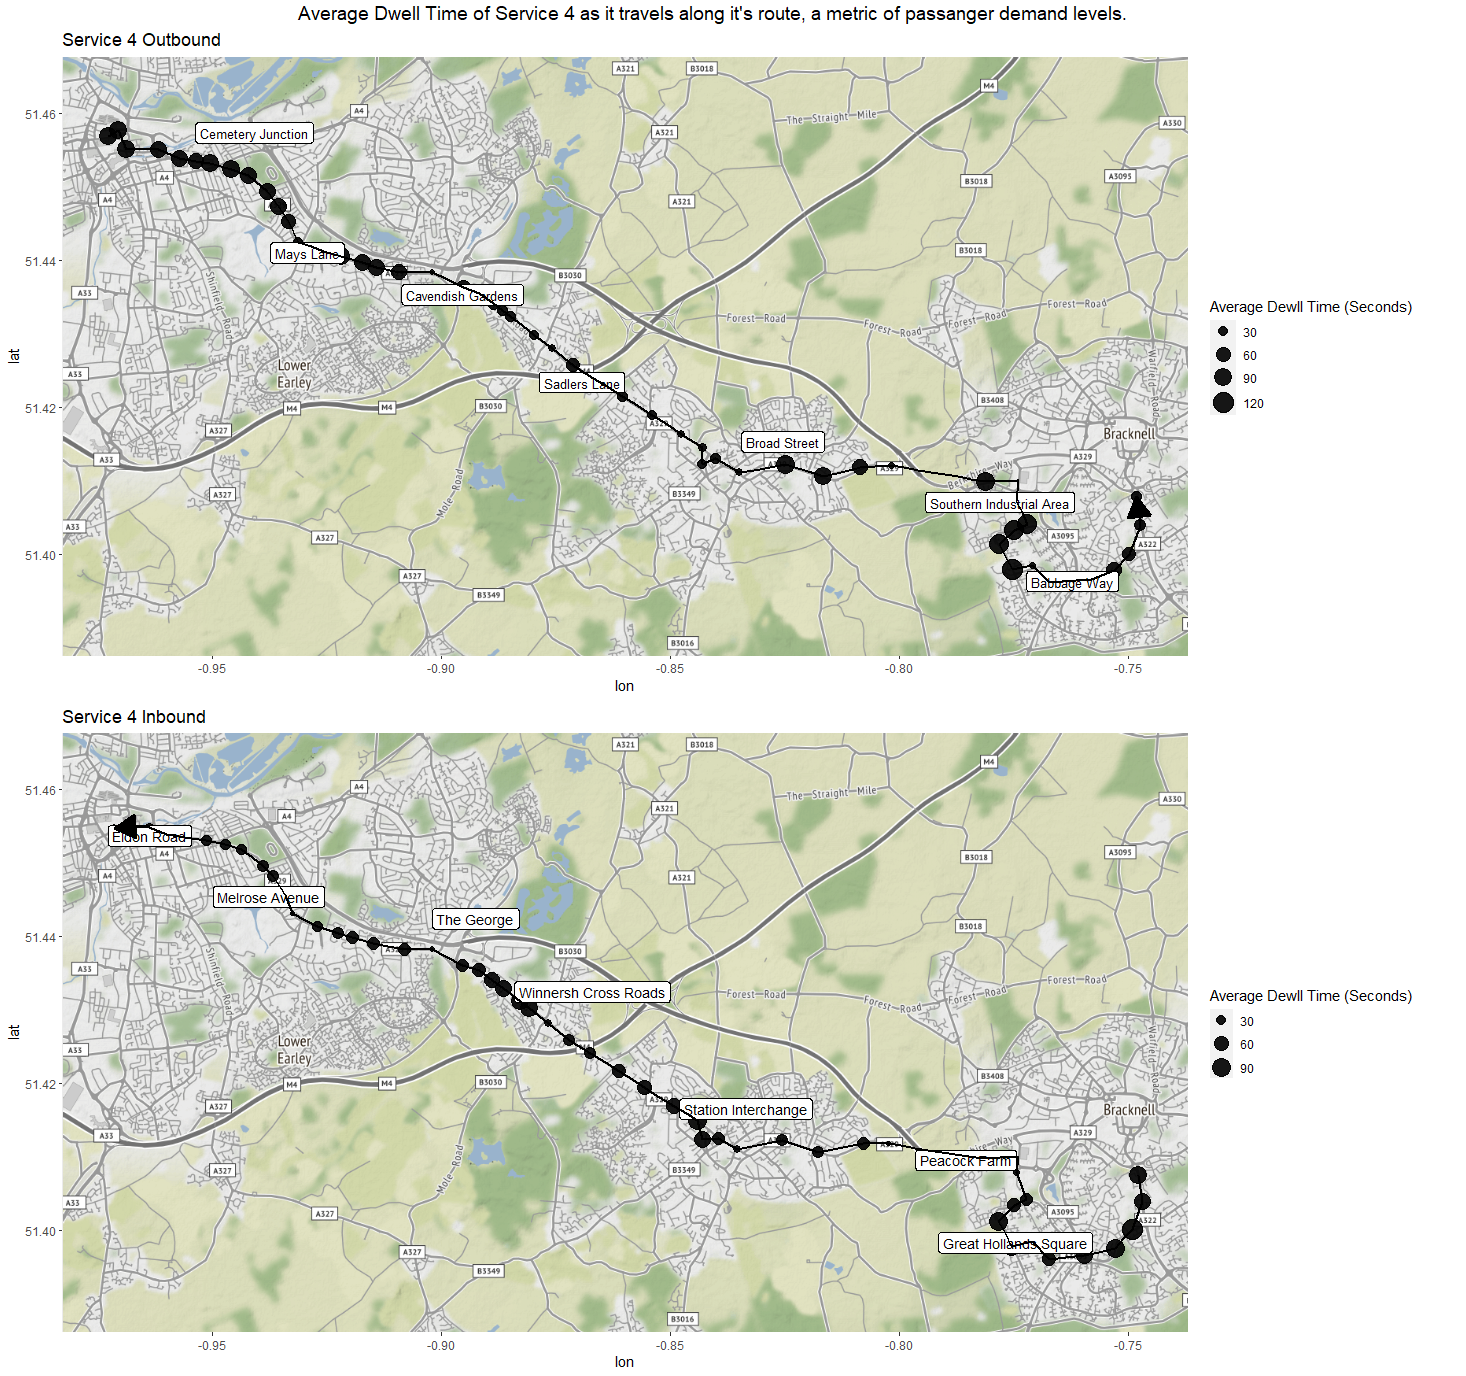
\includegraphics[width=300px]{images/bublechart_4_pair_map.png}
	\caption{Service 4 Average Dwell Time Visualised }
	\label{fig:4dwell}
\end{figure}


\begin{figure}[H]
	\centering
	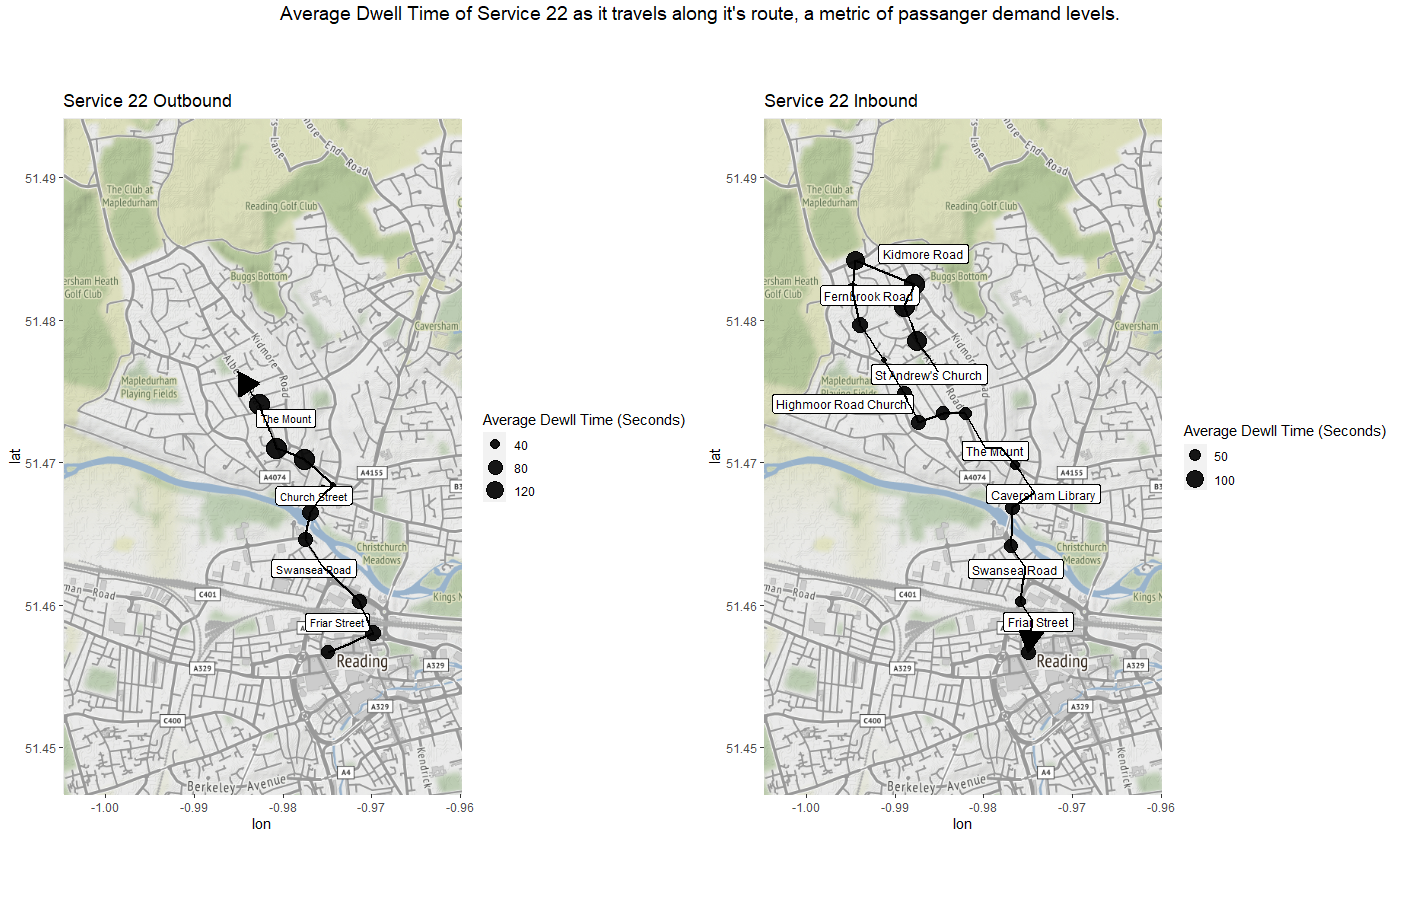
\includegraphics[width=400px]{images/bublechart_22_pair_map.png}
	\caption{Service 22 Average Dwell Time Visualised}
	\label{fig:22dwell}
\end{figure}


\end{document}          
